\documentclass[a4paper,oneside]{memoir}
%		Packages I used to compile this on Ubuntu (found on the ubuntu synaptic repository)
% - texlive-latex-base
% - texlive-fonts-extra
% - texlive-fonts-recommended
% - texlive-science
\usepackage[margin=1.0in]{geometry}
\usepackage{titlesec, color, blindtext, graphicx, listings, textcomp}
\usepackage[vlined]{algorithm2e}
\lstdefinelanguage{CSharp}
{
	sensitive=true,
	morekeywords=[1]{
	abstract, as, base, break, case,
	catch, checked, class, const, continue,
	default, delegate, do, else, enum,
	event, explicit, extern, false,
	finally, fixed, for, foreach, goto, if,
	implicit, in, interface, internal, is,
	lock, namespace, new, null, operator,
	out, override, params, private,
	protected, public, readonly, ref,
	return, sealed, sizeof, stackalloc,
	static, struct, switch, this, throw,
	true, try, typeof, unchecked, unsafe,
	using, virtual, volatile, while, bool,
	byte, char, decimal, double, float,
	int, lock, object, sbyte, short, string,
	uint, ulong, ushort, void},
	morecomment=[l]{//},
	morecomment=[s]{/*}{*/},
	morecomment=[l][keywordstyle4]{\#},
	morestring=[b]",
	morestring=[b]',
}
\lstset{
	backgroundcolor=\color[rgb]{0.95, 0.95, 0.95},
	tabsize=2,
	rulecolor=,
	basicstyle=\scriptsize,
	upquote=true,
	aboveskip={1.5\baselineskip},
	columns=fixed,
	showstringspaces=false,
	extendedchars=true,
	breaklines=true,
	prebreak = \raisebox{0ex}[0ex][0ex]{\ensuremath{\hookleftarrow}},
	frame=single,
	showtabs=false,
	showspaces=false,
	showstringspaces=false,
	identifierstyle=\ttfamily,
	keywordstyle=\color[rgb]{1.0,0,0},
	keywordstyle=[1]\color[rgb]{0,0,0.75},
	keywordstyle=[2]\color[rgb]{0.5,0.0,0.0},
	keywordstyle=[3]\color[rgb]{0.127,0.427,0.514},
	keywordstyle=[4]\color[rgb]{0.4,0.4,0.4},
	commentstyle=\color[rgb]{0.133,0.545,0.133},
	stringstyle=\color[rgb]{0.639,0.082,0.082},
}


\renewcommand{\familydefault}{\sfdefault}

\definecolor{gray75}{gray}{0.75}
\newcommand{\hsp}{\hspace{20pt}}
\titleformat{\chapter}[hang]{\Huge\bfseries}{\thechapter\hsp\textcolor{gray75}{|}\hsp}{0pt}{\Huge\bfseries}

\newcommand*{\SignatureAndDate}[1]{
	\vspace{.4in}
    \par\noindent\makebox[2.6in]{\hrulefill} \hfill\makebox[2.0in]{\hrulefill}
    \par\noindent\makebox[2.6in][l]{#1}      \hfill\makebox[2.0in][l]{Date}
}

\title{\Huge Van Dyke -- Quantum Run}

% List of authors. Update these with your real email addresses.
\author{
	Daniel Bergmann\\
	db0763@my.bristol.ac.uk
	\and
	Matt Bessey\\
	mb0658@my.bristol.ac.uk
	\and
	Bea Domenge\\
	bd0661@my.bristol.ac.uk
	\and
	Joe Lewis\\
	jl0892@my.bristol.ac.uk
	\and
	Callum Muir\\
	cm9757@my.bristol.ac.uk
	\and
	Vlad Otrocol\\
	vo0592@bris.ac.uk
}

\begin{document}
	\maketitle

	% TODO: Write this at the end of the project.
	\begin{abstract}
		We have designed and developed a two player PC game, set in CERN, played entirely via two networked Microsoft Kinects.
		The game consists of one endless procedurally generated level, in which the aim is to survive for as long as possible.
		Game play is cooperative, in that the two players have complimentary skill sets and must work together to assure each others survival whilst being pursued by an antagonist.
	\end{abstract}

	\clearpage
	\tableofcontents

	% This section is done.
	\chapter*{Assessment and Weightings}
		We have agreed to be assessed as a group. Our agreed individual weightings are:

		\begin{itemize}
			\item 1.03 --- Daniel Bergmann
			\item 1.19 --- Matt Bessey
			\item 0.95 --- Bea Domenge
			\item 0.85 --- Joe Lewis
			\item 0.87 --- Callum Muir
			\item 1.11 --- Vlad Otrocol
		\end{itemize}

		\noindent
		Signatures of the group members:

		\SignatureAndDate{Daniel Bergmann}
		\SignatureAndDate{Matt Bessey}
		\SignatureAndDate{Bea Domenge}
		\SignatureAndDate{Joe Lewis}
		\SignatureAndDate{Callum Muir}
		\SignatureAndDate{Vlad Otrocol}

	% I just put in a few temporary suggestions. The lines of code needs to change, it is in fact
	% less than 9000 lines of code.
	\chapter*{Top 10 Contributions}
		\begin{enumerate}
			\item We adopted an iterative design process for all aspects of the game.
			\item We wrote $\sim$9,000 lines of predominantly C\texttt{\#}.
			\item Game levels are procedurally generated at runtime as the player plays the game.
			\item The player moves fluidly through sections, along a Bezier curve generated in Unity based on Maya locators in each section.
			\item Mapped players to the game avatars using multiple Microsoft Kinects.
			\item Streaming player Kinect information over a local area network.
			\item Kinect server runs asynchronously, significantly improving framerate.
			\item Created many sections and models in Maya, which are UV mapped onto the same textures for consistency.
			\item Almost all meshes in the game are original content, created, animated and textured by the team.
			\item Used polymorphism to allow complex sections of the game to be extended from a base section.
		\end{enumerate}

	% 
	\chapter{Introduction}
		% Introduce the game, explaining what it does. 
		% The marking panel will play your game, but assume that they may not have.
		% (5 pages)

		The date is September 10\textsuperscript{th}, 2008, the setting, the bowels of CERN, the European Laboratory for Particle Physics.
		Our protagonist, Professor Anthony Van Dyke sits in his lab monitoring the state of the LHC, which is to be turned on for the first time imminently.
		The world media has spread fears of this moment for weeks, but the scientists know that such here-say does not even bear thinking about...

		Except as it turns out, this time it does. As the LHC is powered up, a tremendous rumble grows from the ground, walls shake and the collider is torn apart before Anthony's eyes.
		He is in a privileged position, for most were instantly vaporised in this tragedy, Anthony however, was split into his matter and antimatter self.
		Blessed with the powers of creation and destruction respectively, it is the job of these two men to save the world from annihilation, for with there powers came something much worse, a monster from another dimension, hell bent on destroying all of reality.

		This is where our game begins. 
		You and a friend take on the roles of the two Anthonys, riding the latest in experimental CERN hover pad technology.
		Your goal is to stay alive as long as you can, guiding the monster away from the LHC, through the labs of CERN, buying the world some time.

		The game is played with full body tracking. 
		There are no controllers, or keyboards, instead the characters mimic your actions exactly, in real-time.
		Your left hand is used to steer the vehicle or aim the gun, depending on your position.
		Your right hand is used to activate your creator or destroyer abilities.
		At any time you can switch between driver or gunner, by both stamping on the ground simultaneously.
		There are some attacks that only one player can deal with, so it is important to communicate throughout to tell your team mate when to switch!

		%TODO umm Would change this, might not go down well
		Breaking the trend in the group games project, this project has run smoothly throughout. 
		We met regularly as a team, for both management and development, all year long, avoiding leaving the bulk of work to the last minute.
		We also met fortnightly with our mentor, Andrew Buchanan, whose advice and most of all outside perspective was very much appreciated, and without which we would not have the game we do today.
		We discuss this further in the following \textbf{Group} section.

		The project has run smoothly, in spite of an overzealous specification in the beginning. 
		We realised over the course what was feasible and what was not, and as such the features that remain have received the time they deserved.
		We discuss how the feature-set of the game adapted over time further in the \textbf{Project Planning} section.

		Since the games length is not fixed, but is instead an ``endless running'' game, the map is procedurally generate on start up and throughout playing.
		As such we have faced challenges of memory management, achieving a consistent art style throughout, and blending together the interlocking pieces of level, to name but a few. We discuss further these challenges, and more, in the \textbf{Technical Content} section.

		Naturally with a project of this size, we ran out of time to make full use of all work.
		This has held particularly true in the Kinect department, where Dan developed a fantastically flexible interface to the Kinect SDK, allowing mapping of complex joint movements and even multiple sequences of joint positions over a timespan.
		Unfortunately these were underused in the final game, but the system is still there, documented thoroughly in the \textbf{Technical Content} section.


	\chapter{The Group}
		% The group process. Discuss how the group worked; what went well and what didn't work. 
		% Have you learned anything about group work - would you change anything about the way you worked if you had to start again. 
		% What methods were employed to assist the group process?
		% 5 pages.

		As a group we have throughout this project continually agreed that, in spite of many hearing many horror stories, this project has run incredibly smoothly. The group gelled well together and there have been no grand personality clashes as members have had in previous projects, and despite its magnitude workload has been spread evenly and taken well by all members. Here, we discuss what enabled this frictionless experience.

		We held regular management meetings, every Tuesday in the MVB caf\'{e}, in which no code was written to ensure focus. 
		These meetings helped ensure a clear, shared vision for the game was held by all members, and that the group's priorities for the coming week was clear. 
		These meetings rarely lasted more than an hour after the first week, and they allowed us to work relatively autonomously for the rest of the week.
		By ensuring that once a week all members were present for the management meeting, it was easy to regularly check on individual contributions, 
		ensuring a fair share of work was being done by everyone every week.
		In addition, it removed any risk of a member wasting their time on unnecessary work because they were not aware of recent developments in other areas of the game.

		In the beginning of the project we discussed issues members had had in previous group projects, and attempted to use this experience to improve the project ahead of us. 
		One unanimously agreed upon point was that the majority of group time should be spent working together, not separately. 
		This was very successful early on in each semester as we had less work commitments outside of the group, but proved to be more of a challenge towards the semester's end.
		Despite this we successfully met all non-holiday Sundays in the MVB, working for 6 hours, consistently.

		For task management, initially GitHub issues were employed, as they tied in nicely with the Source control. 
		The GitHub issues tracker (see Figure ~\ref{fig:GithubIssues}) is fairly standard; tasks with description can be recorded, with a member assigned to them, and comments can be made on them by any member. 

		\begin{figure}[ht]
			\begin{center}
				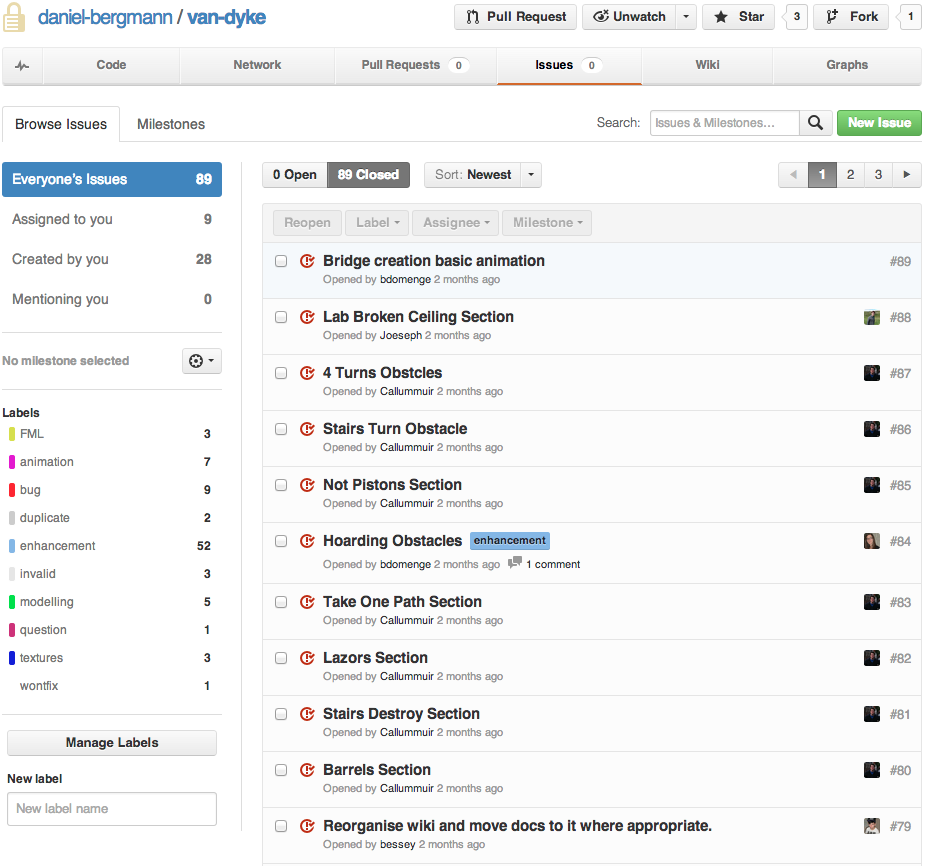
\includegraphics[width=150mm]{../Screenshots/github-issues-home.png}
				\caption{An example page of issues tracked through GitHub}
				\label{fig:GithubIssues}
			\end{center}
		\end{figure}

		Initially this sufficed, however as the breadth of tasks in the system increased, a simple tabular layout made Matt's task of keeping track of the overall project progress more and more difficult. 
		To combat this we switched to a new unusual task management system, Trello. 
		Trello expands on the simple tabular layout of a standard issue tracker by adding a horizontal structure, giving a left to right progress of a task through its life.


		By adding this higher level structure, seeing overall progress was made much easier, Figure ~\ref{fig:Trello} demonstrates our use of it well. 

		\begin{figure}[ht]
			\begin{center}
				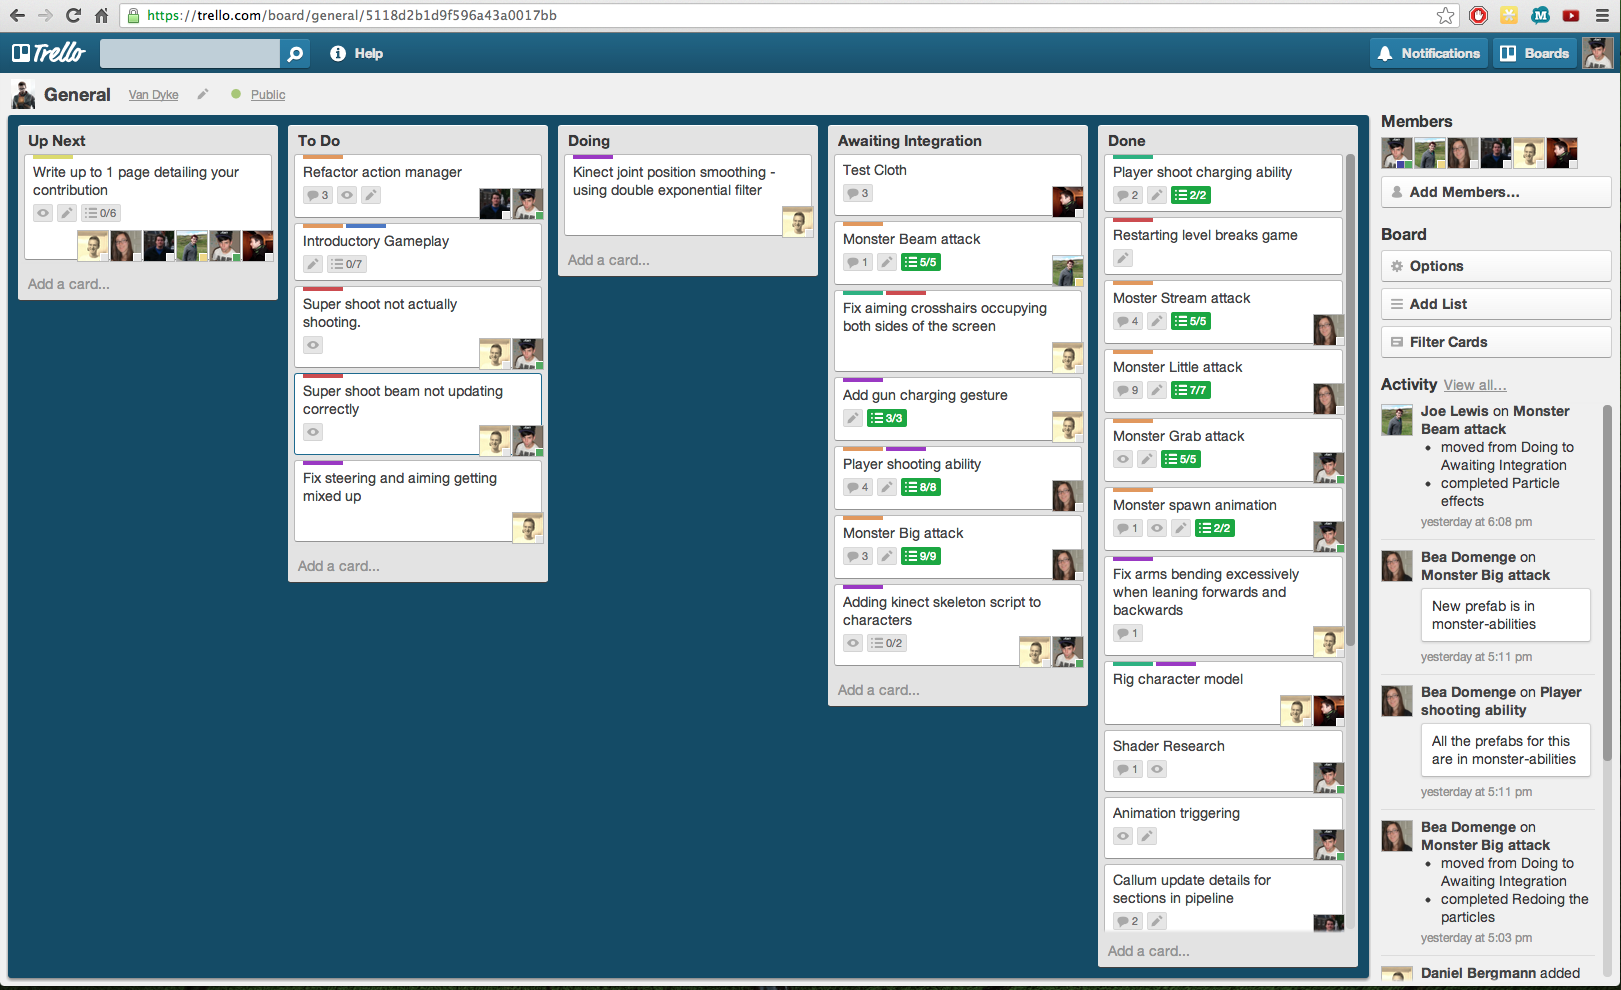
\includegraphics[width=150mm]{../Screenshots/trello-general.png}
				\caption{The ``General issues'' board. Note the left-to-right flow of cards indicating progress.}
				\label{fig:Trello}
			\end{center}
		\end{figure}

		Later on in the project when finding group working time was harder, having a shared point of task management where any member could see what others were up to was incredibly useful.

		A feature of GitHub we did continue to use throughout the project was the wiki services. 
		Even with regular communal working, we found the best way to disseminate and archive knowledge throughout the team was to maintain a wiki. 
		This ensured that in areas where a specific system had to be followed, and was not necessarily programmatic (e.g. in Maya) a guide could be written by one member for all members to then follow.

		\begin{figure}[ht]
			\begin{center}
				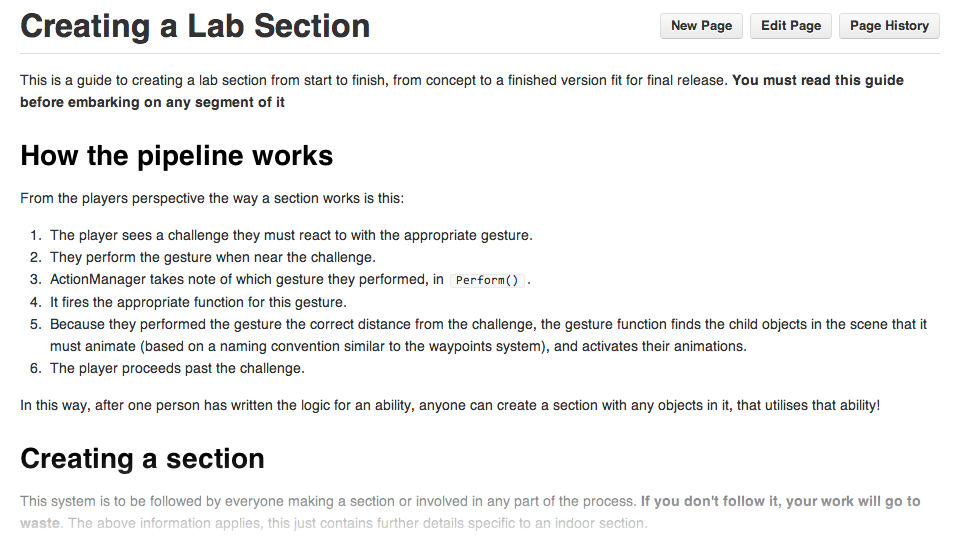
\includegraphics[width=150mm]{../Screenshots/github-wiki-page.png}
				\caption{An example Wiki page written to instruct members how to model a section.}
				\label{fig:Github Wiki Page}
			\end{center}
		\end{figure}

		To ensure group members enjoyed their time spent on the project as much as possible, task delegation was not arbitrary, but based on members preference and skills.
		For example, early on it became clear that Vlad was the Maya champion of the group, as he was enrolled in both Character and Set Design, and Animation Production, simultaneously. 
		As a result, his work was almost entirely Maya based throughout the project. 
		On the opposite end of the spectrum, Callum was the only member not taking Character and Set Design, and as such rather than forcing him to learn new software, he focussed on Unity programming and artwork.
		Similar task to skill-set matching was maintained for every member, and only in times when the workload did not allow preferences to be honoured did members have to resort to work they were disinterested in.

		An important element in any group project is software version control. 
		With six people all coding at once, often on overlapping parts of a project, issues were bound to arise if no thought was given to this. 
		Fortunately, this was recognised early, and practically the first thing our group did when we sat down for our first management meeting was set up a shared Git repository to work from. 
		Not only this but before any commits were made every member followed a learning Git tutorial to ensure correct procedures were understood. 
		Further information on the Git process can be found in the Software section.

		\section{Evaluation}

			Thanks to the aforementioned measures, the project went remarkably smoothly. 
			The combination of Trello and Git enabled Matt to manage effectively, and for the whole team to work concurrently effectively too. 
			Based on our experiences, our inkling on the importance of group work seems very much founded; by far the most effective periods of work we shared were those 6 hour Sunday sessions, where the whole group was present.
			Even when everyone was working on separate tasks, just being able to ask a question ``to the group'' can be so helpful, saving hours of otherwise wasted time on duplications of effort.
			Lastly, as seen in Figure ~\ref{fig:GithubGraph}, these sessions helped ensure we worked on the project throughout the year.
			
			\begin{figure}[ht]
				\begin{center}
					\includegraphics[width=150mm]{"../Screenshots/github-graph"}
					\caption{Graph of our git commits throughout the project.}
					\label{fig:GithubGraph}
				\end{center}
			\end{figure}

			Probably the best example of these systems coming together in full force to enable rampant productivity was during the section creation phase of the project. 
			During the Christmas holidays, with Vlad's Maya advice, Matt ironed out a specification for level sections and a guide to creating them, broken down into the smallest stages. 
			It effectively specified an entire pipeline, beginning with a draft design on paper, and ending with a fully modelled, animated, textured, and scripted level section. 
			This specification took a good day to design and create, and was iteratively improved based on members findings while using it, but importantly it meant that in the period of a fortnight, the bulk of game content was created (though texturing was saved for later).
			Before this stage, content production was slow because no one (including Matt!) was entirely sure on what a section should look like, or how they should piece together.
			After creating a specification, all of the information on how to create a section was clear and on hand, and the team was quick to come up with ideas for challenges the players could face, and then develop them.

		\section{Lessons Learned}

			Naturally, no project comes without problems, and Quantum Run was no exception. While there were few issues throughout the project, we shall cover those that occurred here.

			Probably the most frustrating situation a group can find themselves in when working together is when many members are waiting on the completion of a task started by one member. 
			While this situation rarely arose, when it did, it was chiefly due to Matt acting as both the project manager, and integrator. 
			While this was due to Matt having the greatest knowledge of Git at the beginning of the project, the tool is not too difficult to learn and in hindsight it would have been prudent to assign these roles to two different members.
			After all, every member had to learn to use Git for the project, so any could have managed the repository.

			Next on the list, and an oft repeated pitfall when working in new territory, was to research thoroughly before beginning a task. 
			In the early stages of the section pipeline, shortly after the wiki had been written and the team began working on creating the bulk of the game's model content, there was an unnecessarily large amount of re-factoring of geometry to meet new standards. 
			This is a tricky issue, as it's easy to see in hindsight that the approach settled by the end should have been the one settled on at the start, nevertheless while it is doubtful that we could have avoided all re-factoring, with a little more research from those writing the initial specification we could certainly have avoided some.

			Lastly, one area that members agreed, based on previous sour group project experiences, was an issue that should be tackled from the start and throughout, was team weightings.
			Accordingly we came up with what we deemed a fair system for weighting distribution that accommodated several needs. The system we initially designed had to meet these criteria:

			\begin{itemize}
				\item Iterative; the system should be able to take new information weekly giving a current estimation of weightings.
				\item Work focussed, not time focussed; we believed it was unfair to reward hours committed that weren't useful, especially as hours are far easier to falsify than actual work.
			\end{itemize}

			This seemed like a good idea at the time, however alongside our already thorough organisational measures, this turned out to be massively over-engineered and in hindsight a little pessimistic! 
			Half of every management meeting was spent deciding the value of each members contributions every week, and we soon realised that it wasn't fair to weight work lower when the work was clearly assigned to the member. 
			If two people are given two tasks and they both complete them, which one is harder is irrelevant, they both did what they were asked to. 
			The only metric left after that to measure from was hours, and so our fancy spreadsheet devolved into a much simpler and much preferred time sheet.
			That time sheet, along with all our other management tools, proved to be more than enough.

			In the second semester we had trouble finding time to work as a group. Having got used to our scheduled work sessions we had some trouble adjusting to the new structure of working. 
			%TODO: add to this, check with everyone its cool mentioned enough

	\chapter{Project Planning}
		% Discuss how the planning and time-management process worked. 
		% How closely did you keep to the plan, and in what ways did it change?
		% 5 pages

		When we initially pitched Quantum Run, its working title was Dream Runner, and while its game play was reasonably similar to Quantum Run's, its setting was vastly different.
		We heeded the advice of the panel who essentially warned that dream sequences are very hard to pull off, and brainstormed an alternative setting and plot line for the game.
		After spending an evening brainstorming an alternative setting, we came up with what is now Quantum Run.

		Next up was to decide on an art style, at least approximately. 
		We all agreed that - besides being beyond our abilities - a photo realistic style was not appropriate for the game play we had in mind. 
		After coming to that decision all that was left was to do was narrow down from ``cartoonish'' to a slightly more specific style, so character and level design could commence.
		We perused Colin's collection of game artwork and made a short list of styles we all thought were appropriate for Quantum Run (see Figure ~\ref{fig:MoodBoard}).

		\begin{figure}[ht]
			\begin{center}
				\includegraphics[width=120mm]{"../Screenshots/Early Research/mood-board"}
				\caption{Our assembled mood board}
				\label{fig:MoodBoard}
			\end{center}
		\end{figure}

		While the range was still fairly broad, a reasonably consistent style became apparent; a rich and bright colour scheme with a focus on simple gradients and subtle textures.
		With this in mind, it was time to select a game engine so we could begin development.
		
		As none of us had significant programming experience in any game engine before this project, we thought the most prudent thing to do was to build a shortlist of popular first timer game engines, and each go away and research a couple of them. These are the results of that research:

		\begin{itemize}
			\item Unity: Can use the official Kinect SDK via interface layer. Very popular first timer choice, a lot of ``for free'' scripts thanks to a large community with StackOverflow style Q\&A site. Not exceptional graphics but more than enough for our needs. Runs on everything.
			\item Ogre: Supports the Kinect SDKs, has good documentation, appears to be difficult to setup but not too bad after that. However it is just a graphics engine, so another engine would be needed for physics, such as Bullet.
			\item Unreal 3: Very nice level designer, similar to Unity's, Kinect support through the Faast library, but we are unsure how powerful this is compared to the official SDK. Strong community and thorough documentation. Incredible at photo realistic graphics, but unclear whether it is capable of cartoonish style.
			\item Source: Multi platform, and very widely used in multitudes of game genres. Huge community. Cartoon renderer ability as evidenced by Team Fortress 2. Every game is essentially a mod for a source game however, lower level integration with the engine not possible without a license.
			\item IDTech 5: Predominantly used for First Person Shooters. No Kinect support however.
			\item CryEngine: Amazing documentation with video tutorials and more. Large and active community. Kinect support implemented by CryTek themselves. As with Unreal 3, no question this can do incredible photo realistic graphics but not sure on its cartoon ability. Again seems focussed on first person shooters.
			\item Frostbite 2: Unattainable; only for large game studios.
		\end{itemize}

		It was a close call between Unity and Unreal 3, however, Unreal 3's system requirements were such that Dan's laptop simply could not open the level editor, with this the decision was made a lot easier. We pressed on with Unity.

		% TODO: Dan you might want to comment more about the pros and cons here, as I am not qualified. - Matt
		While doing this initial research we also took the time to learn more about our options for interfacing with the Kinect. The two clear choices were the Microsoft SDK, and OpenNI.

		For early decisions like game engines and Kinect interfaces, it made sense for the entire group to consider the options and decide on the best together, given their sheer importance.
		However, for more artistic decisions we did not believe that 6 people meant 6 times more creativity than a single member coming to decisions, but rather would end in some ungodly amalgamation of 6 nice ideas into a single watered down compromise.
		In such situations, creative control was left to the member assigned the task, with some feedback from the group to ensure nothing to outlandish.
		And in this way, the monster, player, vehicle, and general lab aesthetic were designed (see Figures ~\ref{fig:FinalProfessor} and ~\ref{fig:ColourScheme}).

		\begin{figure}[ht]
			\begin{center}
				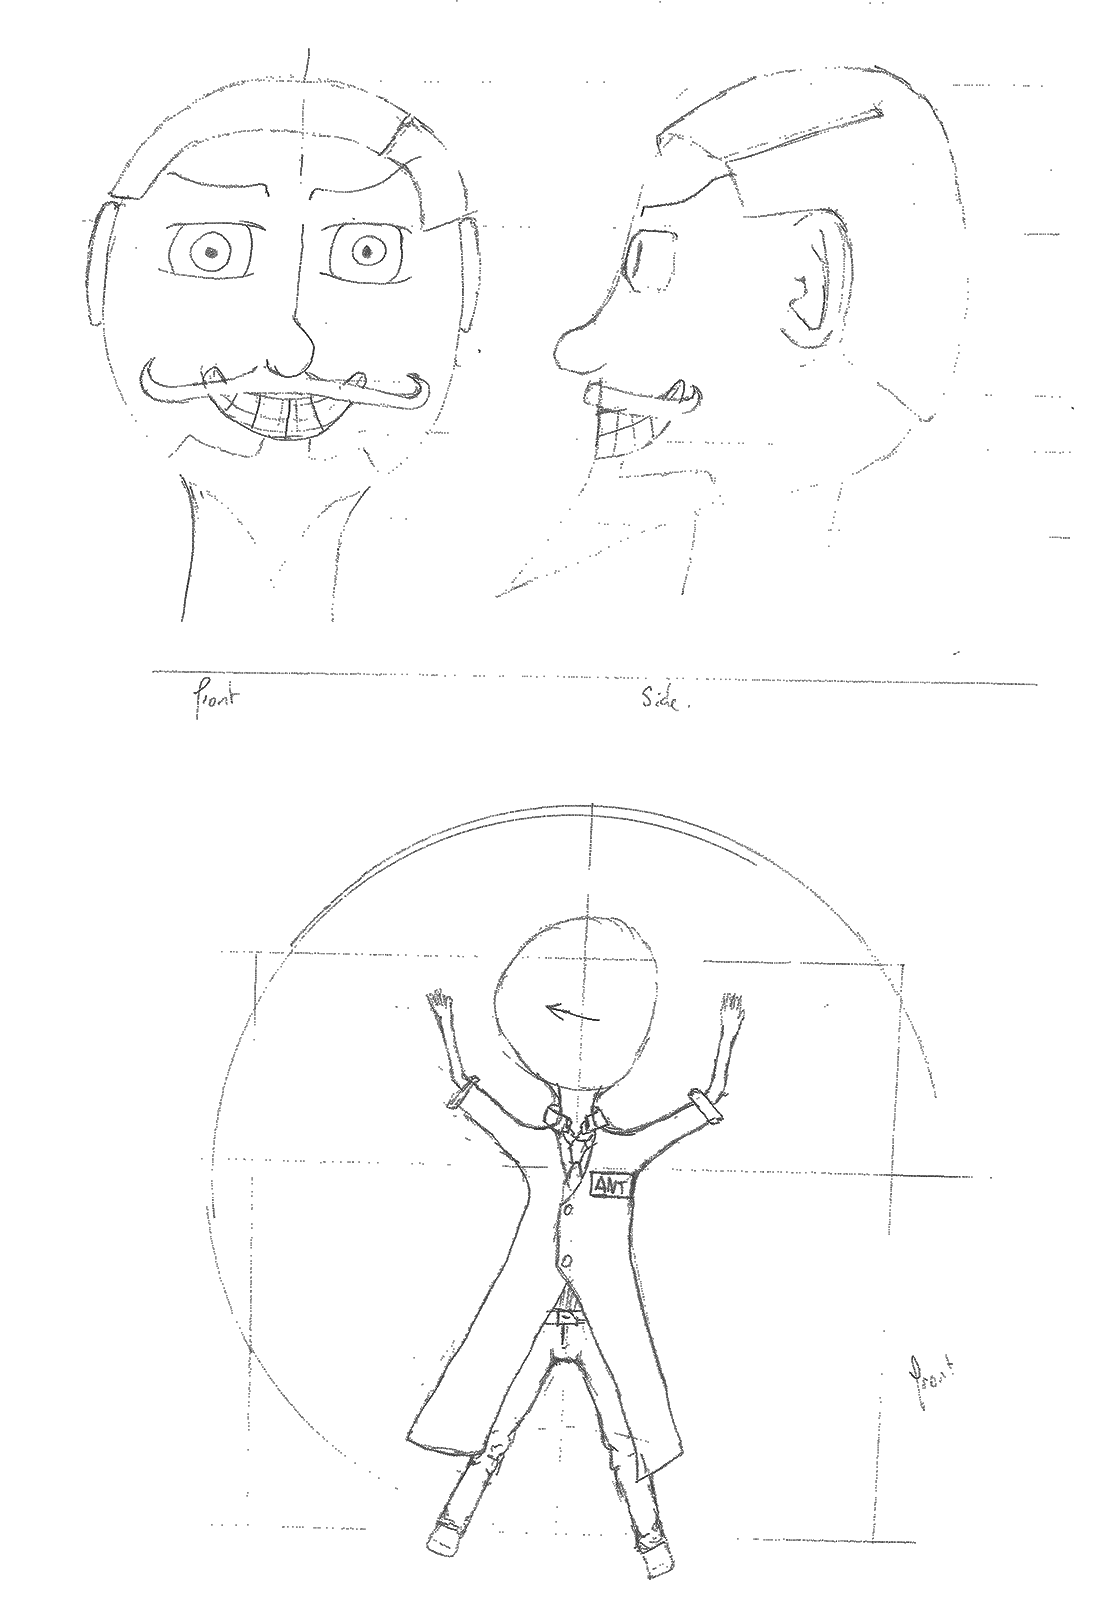
\includegraphics[height=120mm]{../Screenshots/Artwork/van-dyke-final.png}
				\caption{The final artwork for the professor character.}
				\label{fig:FinalProfessor}
			\end{center}
		\end{figure}

		\begin{figure}[ht]
			\begin{center}
				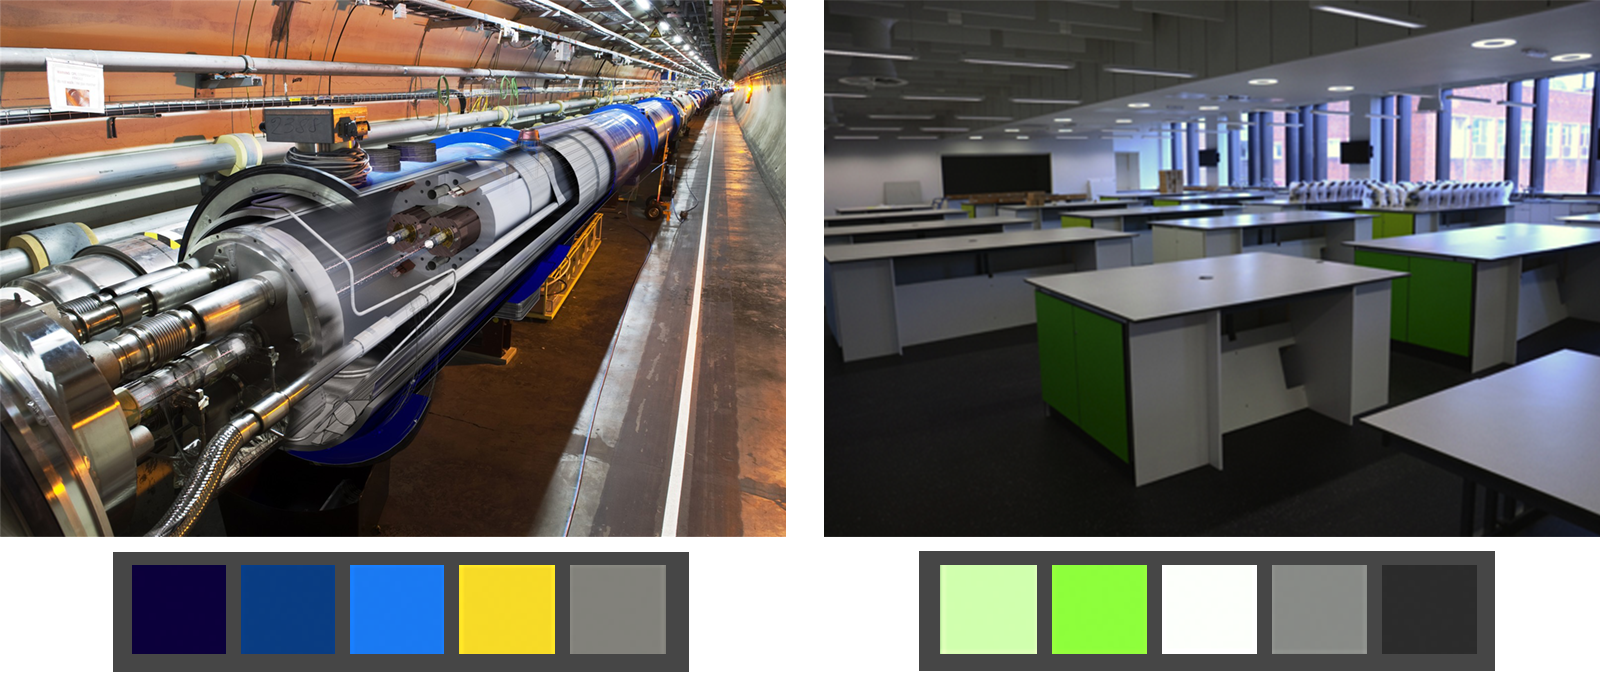
\includegraphics[width=120mm]{../Screenshots/Artwork/colour-scheme.png}
				\caption{The colour schemes used to design the lab and LHC levels.}
				\label{fig:ColourScheme}
			\end{center}
		\end{figure}

		Constant steady progress was maintained throughout the project, thanks to our regular meet-ups. However progress was fairly slow, and after a meeting with our mentor, Andrew Buchanan, on his advice we decided to start a process of self enforced fortnightly deadlines.
		These worked well, not just to improve throughput, but to distil what the most important features of the game were.
		Picking tasks to focus on for the next deadline was easy; we simply asked ``If we had to demo the game today, what feature would be most important?''. 

		Half way through the project, it became clear our specification for the game was too ambitious, in that our original plan to have 3 ``levels'', or themed sections, wasn't achievable in the timescale. 
		As a result we decided to distil the game into the one themed section we were planning on starting with; the indoor lab level. 
		It was thanks to noticing this relatively early on in the games development cycle that we were able to avoid wasting time and effort on the other levels.

		Toward the end of the project, around March, it became clear we weren't going to be able to include the intended game mechanics in a satisfactory form. 
		While the functionality for front \emph{and back} special abilities was already implemented, we only had two sections that made use of the back players abilities. 
		Since the back player already has a reasonable amount of gameplay, involving shooting at monster projectiles and relaying information to the front player, it wasn't a difficult choice to remove this further gameplay for the sake of the quality of the remaining game features.
		In retrospect, it would have been sensible for us to have implemented, as a group, one game mechanic at a time, play-testing between each one. 
		Instead many were implemented in parallel, giving little opportunity to re-evaluate future goals, and ultimately ending in wasted work on gameplay that could not be used.

		\section{User Testing}
			Throughout the project we had struggled with user testing, not because we were reluctant to do it, but because our hardware requirements were so specific, setup and tear down time alone could take half an hour.
			As a result of this, testing was only really done with keyboard commands emulating Kinect gestures, which it turned out is a very different and much easier input method.

			When we came to do our first user testing with participants that hadn't been involved in game development from an early stage, one issue became very apparent; our control system was far too hard!
			Every play test started with us spending a good five minutes baffling the players trying to explain that there were two control systems, one for each character, but also that you could switch which character you were, so you still need to learn both.
			On top of this, players' default ``I have no idea what I am supposed to do'' action was invariably to throw both their hands in the air.
			This would result in the players switching places, confusing the players even further, and while amusing for all involved, it was not desired gameplay.
			At this stage we made the decision to turn this behaviour into a positive, we concluded that if we remapped the player's primary ability to raising their hand, in the majority of cases a confused player's default reaction would actually be the correct action too.
			We also decided at this stage to combine the remaining two abilities of the front player into one, to remove one more control to learn. 
			This meant that we could distil obstructions for the driver to overcome into three categories; ``things I can avoid'', ``things I can deal with by raising my hand'', and ``things my partner can deal with by raising their hand''.

			Of course in hindsight the signs were there throughout development that the game was too hard. 
			Whenever we were play testing the game, \emph{the game we made}, rather than playing through properly we would found ourselves hammering every ability key knowing one of them must be right.
			Initially we believed each player should have \emph{four} abilities activated with \emph{four} distinct gestures, or the game would be too easy.
			We believe that fear stemmed from previous experience with puzzle games played with a controller, and indeed that seems to be the lesson to take away here; you cannot remap a game pad's controls onto a person, and expect them to be able to play as effectively as they could with a controller.

	\chapter{Individual Contributions}

		We attempted to divide the workload as evenly as possibly whilst balancing individuals preferences and strengths.

		\section{Daniel Bergmann}
			
			From the start my main role was programming the Microsoft Kinect to be used with our game.
			I was almost entirely responsible for all the code related to the Kinect. Some other members, mainly Matt assisted in parts of the integration and we all discussed as a team what features we wanted for the Kinect as well as constantly re-evaluating how things were progressing with it but I was the person who was delegated to implement all of this. The main areas I worked on during the project were:

			% This is an unordered bullet point list. Each item on the list is preceded by the \item
			% mark up.
			\begin{itemize}
				\item Research existing Kinect--Unity interface libraries and Initial skeleton tracking with 3\textsuperscript{rd} party library\cite{Kinect::Adevine1618} --- 60 hours
				\item Created external Kinect program to interface with Unity to stream skeleton data over either the local loop-back address or over a local area network. --- 40 hours
				\item Kinect-Unity integration on Unitys side with KinectSkeleton script for in game models. --- 100 hours
				\item Kinect gesture control and mappings. --- 50 hours
				\item Avatar Mapping with Joint Rotation. --- 100 hours
				\item Brief look at JSON serialisation in C\texttt{\#}. --- 10 hours
			\end{itemize}

			% A subsection is just the next level of division down from a section. Inside your
			% 1 page this is the highest level block you should use. Next down from subsection is
			% subsubsection.
			\subsection{Researching Libraries and Initial Unity Plugin}


				Initially I used a 3\textsuperscript{rd} party library to interface with the Microsoft Kinect and Unity, as the version of C\texttt{\#} used by the current version of Unity does not yet have support for the Kinect SDK. The library I used provides player position data for one player. Using this I was able to create the basic functionality to map joint position data to an avatars joint positions inside the Unity Engine.


			\subsection{Kinect Skeleton Data Server}

				After discovering that the Kinect/Unity plugin did not provide joint information for two players I opted to create an external C\texttt{\#} program to access the Kinect SDK (hence forth known as the Kinect Skeleton Server) and stream the data to our game application. This was convenient because I wrote the external application using the latest version of C\texttt{\#} to access the Kinect SDK. To communicate between the Kinect Skeleton Server and our game I used network sockets programming with multiple concurrent threads, one thread responsible for each stream of player data communicating over different ports.

			\subsection{Implement Kinect gesture control}

				I was responsible for creating the Kinect gesture control and wrote all the related classes to this include the \texttt{JointConstraint}, \texttt{Gesture}, \texttt{AnimatedGesture} and \texttt{Mapping} classes which I have outlined in detail in the technical section of the report. The gesture control is used to control the game through gestures from the players. Gestures loosely to mean physical positions of the body which have a meaning in game, however I use the term gesture in a more strictly defined sense in the technical section.

			\subsection{Avatar Mapping with Joint Rotation}

				I implemented the mapping of joint rotation data to the in game avatars including writing all the code to calculate joint rotations from joint position data.
				As well as this I spent a significant amount of time researching the Microsoft Kinect SDK bone orientation as well as trying to integrate this with Unity.
				The problem of Avatar Mapping is a difficult one which I think we have solved reasonably well.
				I investigated quite a lot about filtering with the Kinect as well, however I did not implement much filtering as I had more important features on my todo list.

			\subsection{JSON serialiser for C\texttt{\#}}

				I looked at this briefly, and in that short time wrote code to serialise all the gesture classes to a JSON file from scratch (the old version of C\texttt{\#} in Unity doesn't even have the C\texttt{\#} serialisation libraries included which I find appalling).
				However in order to successfully reconstruct the objects from the JSON files, I would have had to write a JSON parser which I could do but I had much more important tasks to do in the group.
				Setting the gestures just by constructing objects in a C\texttt{\#} initialisation function was more than sufficient so we dropped the JSON serialisation.

		\section{Matt Bessey}
			% Up to one page describing the main tasks you undertook for the group.
			% use my paragraph above as a template or to see how to roughly use latex

			My primary roles in this project were team leader, integrator, and lead developer. My areas of focus were:

			\begin{itemize}
				\item Group management. --- 50 hours
				\item Version control. --- 50 hours
				\item Set and documented standards. --- 50 hours
				\item Final section manager design and implementation. --- 50 hours
				\item Dynamic tutorial system. --- 25 hours
			\end{itemize}

			Though it is worth noting I estimate I have spent another 100 hours combined on other smaller tasks.

			\subsection{Group Management}

				To make coordination simpler, at an early stage of the project I was (democratically) elected to be group leader. This has meant writing the agenda for our weekly Tuesday management meetings, ensuring all members have done a respectable amount of work, have more work to do, and are not stuck or using their time ineffectively. Lastly it of course meant I was generally the ``go to person'' when a team member had a query. 

			\subsection{Version Control}

				From the beginning and throughout the project we used Git for software version control. Since I was the member with the most Git experience, it was left to me to coordinate integration of branches into the master branch. This meant not only conflict resolution, but also manual merging of the binary files that Unity stores scenes in.

			\subsection{Set and Documented Standards}

				By the end of the project our personal wiki stood at 3,500 words, predominantly written by myself. In areas where strict coordination was paramount, such as section design and development (where each section must interconnect both programatically and literally in 3D space), I took the time to research best practices and decide on standards for the group to follow. By assigning this task to one member, we were able to ensure there was relatively little wasted effort as the standard for all work was explained from the start.

			\subsection{Section Manager}

				The Section Manager is responsible for the procedurally generated map spawned and continuously updated on each run of the game. A simple version was initially created by Vlad, but as section designs became more exotic, with turns and falls, and multiple levels, it became clear a more powerful manager was needed. I designed and implemented this second iteration of the section manager. It's features include: 

				\begin{itemize}
					\item Understands and keeps separate the Lab and LHC levels.
					\item Can interconnect any two sections from each level.
					\item Can transition between levels using special sections.
					\item Handles six degrees of freedom in all sections.
					\item Ensures multiple consecutive resulting in overlapping sections cannot occur.
					\item Spawns sections continuously as the player travels forward.
					\item Deletes previous sections continuously as the player travels forward.
				\end{itemize}

			\subsection{Tutorial System}

				I created the tutorial system used throughout the game, when in tutorial mode. 
				The system was designed to handle the dynamic nature of the game, such that no extra content was required for the tutorial.
				Since this means players could be in either position whenever a tutorial is fired, the system had to take this into account.
				For example, if the driver is approaching a floor that needs restoring, but the creator is currently not the driver, the tutorial system must still notify the creator, so they know to turn around.
				As well as this, each tutorial must show exactly once, the first time it is needed, but never again after that.
				I accomplished this using a hash table which stores with each tutorial pop-up, whether that pop-up has been shown before.

		\section{Bea Domenge}
			% Up to one page describing the main tasks you undertook for the group.
			% use my paragraph above as a template or to see how to roughly use latex
			My main responsibility was content creation for the game, I worked on:

				\begin{itemize}
					\item Modeling and designing game sections. --- 50 hours.
					\item Modeling and searching for game obstacles. --- 100 hours. 
					\item Modeling and designing Player abilities. --- 130 hours.
					\item Particle effects and animations for Player and Monster Abilities. --- 30 hours.
					\item UV mapping sections. --- 25 hours.
				\end{itemize}

			\subsection{Game Sections}
				Initially I worked on researching how we could get the player to move along waypoints in unity, I managed to get the basics implemented, which Vlad then built upon to create our current system.
				Once the method by which sections are procedurally generated became clear, Joe and I worked on modeling sections that had been designed by Callum, at first this involved very simple sections that were made up of straight pieces or turns. During this process the standards needed to create sections consistently were changed several times until the best system was found. Once the sections designed by Callum were all modeled, Joe and I then designed and modeled more according to the pipeline set up by Matt.

			\subsection{Game Obstacles}
				The empty game sections that had been created needed obstacles, at this point we knew that we needed lots of content, at first I modeled some objects, such as a CERN ``buggy'' and a vending machine.
				Then I spent quite some time finding suitable free models online, downloading them and then changing them to be used in the game; this involved lowering the poly count or making sure the object would match the agreed upon aesthetics.

			\subsection{Player Abilities}
				Basic ideas for player abilities had already been discussed with Callum, but Joe and I needed to sit down and work out section / obstacle designs that would match the suggested abilities.
				During this process we also thought of new abilities and obstacles that would enhance game play, for each ability we designed a section or sections that would require the use of the ability and then, once they were approved, modeled them.

			\subsection{Particle Effects and Animation}
				Once the Monster abilities were scripted, they consisted of grey shapes being fired at the player, I added particle effects for the Monster's big, little and stream attack, as well as adding animation to the little attack. While implementing particle effects, I also did the scripting for the Monster's big attack. 
				I was also involved in adding particle effects to some sections.
				Animation was necessary for the Player abilities, sections would need walls or floor that restored, or pipes that burst when the Player performed a specific action, but as well as this there are sections that contain obstacles that move that the player need to avoid.
				I did the animation for a set of moving layers, and opening doors that need to be avoided by the player.

			\subsection{UV Mapping}
				Once the sections had been created and finalised, they needed to be UV mapped, this was quite a time-consuming task considering the number of sections, however the final result is very pleasing.

		\section{Joe Lewis}
			% Up to one page describing the main tasks you undertook for the group.
			% use my paragraph above as a template or to see how to roughly use latex
				My role in this project was mainly creating the world for the game, I focused on:

			\begin{itemize}
				\item Designing and modelling sections --- 50 hours
				\item Designing and modelling player abilities --- 100 hours
				\item Animating sections with player abilities --- 150 hours
				\item UV Mapping and texturing sections --- 40 hours
			\end{itemize}

			\subsection{Designing and Modelling Sections}

				When it was time to start creating challenges and abilities, Bea and I spent time building basic sections which had been designed by Callum. This took a while as we needed to set standards for all sections to adhere to and these standards changed several times, forcing us to go back and alter sections we'd already completed. When Bea and I had finished the sections Callum had designed, Bea and I designed and modelled some more ourselves. Originally we produced a lot of sections that were plain with no challenges to allow us to get used to the standards, but soon we had to move on the creating sections with challenges to create actual gameplay. 

			\subsection{Designing and Modelling Player Abilities}

				Concepts for player abilities had already been thought about by Callum, but we needed to translate these concepts into section designs. We tried to come up with as many different sections as possible for abilities, we even came up with a few more in the process, and then we modelled them once they were approved. This whole process was made into a very efficient pipeline by Matt.
				We tried to design as many sections as possible for both the creator and destroyer characters, as well as different sections for both rear and front gameplay, before it was decided that the rear player would only be a shooter and deal with the monster rather than have sections with challenges as well. Consequently, some of the sections Bea and I modelled and animated didn't make it in to the final version of the game. There were a lot more abilities for the players in the beginning, however coming up with ideas for sections was very difficult and it proved to make the game overcomplicated for the users. So the powers were eventually whittled down to one ability for each character which can only be used while driving.

				
			\subsection{Animating Sections}

				As Vlad was the only person to have taken Animation Production so initially he took over the animation but it soon became clear that it was going to be too much. So he taught Bea and I the basics and when there was something that he would be able to do quicker than either of us he would do it.
				I worked on animating the sections that I had previously designed and modelled, such as the restoring staircase and ceiling sections, as I knew them best. After the sections were animated it was very easy to script them into the game and test them to ensure that the speed and timings were right. Occasionally I would go back and redo a section's animation if Matt didn't like it or thought it could be improved, this allowed me to learn several new techniques in Maya.

			\subsection{UV Mapping and Texturing Sections}

				All the sections are UV mapped onto two different texture maps, for the Lab and LHC levels respectively, this allowed Bea and I to map the sections on to a template which literally had Wall, Floor, etc. written on them so that Matt could create the actual texture file and simply rename it. Although it was repetitive, it needed to be done and once it was I was quite pleased with the result.

		\section{Callum Muir}
			% Up to one page describing the main tasks you undertook for the group.
			% use my paragraph above as a template or to see how to roughly use latex
				I was responsible for two main sections of the game development. 
				Concept art for the character and locations along with an outline for the abilities and locations, and for gameplay implementation. 
				These lined up quite nicely in the development process, as by the time the concepts and plans were complete there was plenty of gameplay assets to create game sections with and at this point all of the concept art was complete and the gameplay abilities had a robust first draft. 

			\begin{itemize}
				\item Character and Vehicle Design --- 30 hours
				\item Section Design and Implementation --- 150 hours
				\item Gameplay Management --- 150 hours
			\end{itemize}

			\subsection{Character and Vehicle Design}

				Working with feedback from the group as to the art direction I worked on prototype concept art for the player and for the monster, this involved the quick prototyping of designs before producing a final cross section design for Vlad that would be used as the base of modeling the character and vehicle. 
				I also produced concept art for the environment. 
				Throughout this I also worked on how the player and monster would interact, both with each other and with the environment.  

			\subsection{Section Design and Implementation}	

				The game is made up of sections of gameplay procedurally put together to keep the game fast paced with numerous obstacles. 
				Sections needed designing with a main obstacle that needed navigating. 
				These needed to range from simply moving out of the way to having to switch partners and using an ability. 
				I designed the majority of the sections and worked out how the gameplay would work. 
				In tandem with Joe and Bea we created the sections, they mainly creating the models and me mainly creating the gameplay in Unity and coding the obstacles.

			\subsection{Gameplay Management}
			
				We originally had the gameplay working from one class, Action manager, this dealt with every eventuality of what could happen in each section. 
				However as the number of sections grew, and the complexity of the sections increased, we started with the easiest sections to hammer out a workflow, this class was getting unwieldy. 
				I discussed with Matt about this and after a little research we decided to use polymorphism, keeping a base class that dealt with all of the common parts in sections, and then extending this class for all of the special cases. 
				This worked well making it much easier to deal with the gameplay interactions. 
				It was interesting to use a programming method to solve a management issue. 
				I was also responsible for other miscellaneous work in Unity and scripting such as our early attempts at a custom camera controller, which was abandoned early on in the project as a much simpler implementation gave 90\% of the functionality and freed me up to work on the section design.	

		\section{Vlad Otrocol}      
	     My role in this project was to create the dynamic level generation, the characters and the vehicle:

			\begin{itemize}
        \item Dynamic level generation --- 60
		    \item Modelling, rigging, animating and texturing the main characters, the vehicle and the monster. --- 290
        \item General research and setting standards --- 30
			\end{itemize}
            
            \subsection{Dynamic Level Generation}
                
                At the beginning of the project I worked on the dynamic level generation. I set up a system to generate sections such that they form a fluid path for our player to follow. Very soon it became clear that this task was strongly connected to the path generation task, therefore me and Bea collaborated to create the first draft for a working game on rails. There were many challenges as this was happening at the earliest stages of our project, therefore the learning curve was very steep and the approaches we had to different problems quickly changed. This system has been improved throughout the first half of the project, but as the game advanced I moved to solving Maya related issues.
                
            \subsection{Game characters}
                
                Having the most experience with Maya and CG in general it was quite clear from the beginning that I would be in charge of the content creation, which we suspected would be an important part of our gameplay. I was in charge of creating the main characters, the vehicle and the monster from start to finish. This involved:
                \begin{itemize}
                    \item Customizing the Maya interface and generating useful scripts
                    \item Modelling
                    \item Rigging
                    \item Weight painting
                    \item Animating
                    \item Texturing
                    \item Exporting/Importing
                    \item Cloth Simulation
                    \item Particle effects
                \end{itemize}
                
            \subsection{Research and Standards}
                Being the first one to have contact with Unity when researching game engines, gave me an advantage in terms of familiarity with the features, therefore along the project I was the one who investigated new areas such as: importing/exporting, particles, physics simulations, light baking etc. I also documented most useful information I found and later distled it into standards such as Maya standards, coding standards, useful tips etc.

	\chapter{Technical Content}
		% Choose some of the more interesting/challenging/novel aspects of the project to discuss in detail. 
		% Explain why they are technically interesting or challenging and discuss how the problems were overcome. 
		% (10 pages)
		% A successful game will:
			% Have several technically interesting challenges which have been overcome, and explained succinctly, including a good software development tools and techniques.
			% Be playable with little or no training, but have enough depth to satisfy an experienced gamer. 
			% Have come from a development team who have demonstrated a willingness to address problems in the team and have found solutions to them. 
			% Have a relevant look and feel (creative content creation) and be novel.

		\section{Modular Level Design} 

			Because Quantum Run's gameplay is naturally linear, we wanted to find a way to ensure that no two player experience were the same, so players could not just memorize the game.
			To accomplish this without having to spend inordinate amounts of time on content creation, we decided to opt for a modular level design.
			In this system, rather than designing the entire level from start to finish, it is broken down into sections.
			These sections can be stitched together in any order, and indeed are randomly ordered on each play through, ensuring an unpredictable and unique experience on every play through.
			Creating this system raised some interesting technical challenges, which we will discuss here.

			The first challenge we found was decided how to interconnect pieces. 
			Our solution to this problem was to have all section Maya models start at the origin, and mark their endpoint with a Locator. 
			This solution was particularly good because Locators have six degrees of freedom, meaning successive sections can look at a locator's position \emph{and rotation}, allowing sections to turn, flip upside-down, and more. 
			Time constraints meant we did not fully utilise all these possibilities, however you can see that left and right rotation is put to good use in turning sections, as is Z position, in sections where the player goes up or down a storey.

			Unfortunately while Unity has vertex snapping in editor mode, having the engine snap sections together such that there was no gap or overlap between them was not possible. 
			Initially we tried deliberately adding a generous overlap between sections but this led to peculiar artefacts as successive levels textures flickered above and below each other.
			In the end we found overlapping sections by a tiny amount was the easiest solution.

			While random section ordering worked fine for most cases, we found one problem; sections could cross their own path, due several to successive turns in the same direction. Keeping count of how many turns have occurred was not a solution, since there is no rule stating a section must turn exactly 90 degrees, so instead we redesigned the \texttt{SectionManager} class to keep track of the exact rotation of the ``tail'' of our section list.
			With this information, when a new section was to be added, the \texttt{SectionManager} appends the section, looks at the new rotation, and if it is greater than $\pm90^\circ$, it will instead choose a different section.

			Dynamic instantiation itself lends some potential performs problem if not handled sensibly. 
			When the player starts the game, the ``track'' ahead of them is generated to a reasonable distance, ensuring they cannot see off of the end.
			As the player progresses, we simultaneously de-instantiate sections behind them, and instantiate new sections ahead. By de-instantiating sections behind us, we ensure the game's memory footprint does not creep up over time. 
			To ensure as little garbage has to be collected as possible, we use modulus arithmetic on a fixed length array of sections, such that a newly instantiated section will overwrite an old one in memory, without any allocation or deallocation required.
			Using this approach, we found we were able to run the game at $\sim$100x speed without any performance issues.
			This method did mean that we had to keep all of action of the game in this section. A common bug was when actions took place elsewhere in the map, causing the section around to player to de-instantiate. 
			We also had to use the player's location as an event to run animations in some sections. 
			%TODO check above statement

			Once section position and geometry was implemented, the next step was texturing.
			Since we have 20 sections, and the modular design should not impact performance, we wanted to ensure all sections where possible used the same texture file.
			In order to accomplish this, every section had to be custom UV mapped onto the same texture, one that deliberately contained all possible ``pieces'' of wall, ceiling, and floor texture.
			This was no small feat, but over the course of a fortnight and with half the team working on it, we moved all geometry to the new system.
			This approach had the added benefit of meaning, once all sections were mapped, we could tweak their colour scheme as we saw fit in a matter of seconds, and watch the results cascade through the entire game, making consistent design throughout the game trivial.

		\section{Use of the Microsoft Kinect}

			One of the key features about our game is the Microsoft Kinect.
			It is the only form of player input that the game receives and is surely one of the defining features which people will remember when playing the game.

			\subsubsection{Integrating the Kinect with the Unity Game Engine}

				The first challenge of using the Kinect was integrating it with the Unity game engine.
				The problem was that there aren't really any freely available plugins for Unity to allow Kinect support.
				There is the ZigFu plugin which is supposed to give excellent Kinect support in HTML5, Unity and Flash which was even free in it's early days (up until about 2010) but they must have decided there was more money to be made in selling the plugin.
				At \$200 for a developers license we had to look elsewhere.
				Next there is the ``Kinect SDK-Unity3D interface plugin''\cite{Kinect::Adevine1618}, a free to use plugin which seemed perfect and which we actually used for several months to interface between Unity3D and the Kinect.
				However it became apparent that it was unsuitable when we discovered that it did not correctly support two players.

				These were the two most suitable looking plugins available for Unity and the reason why there aren't any others is because Unity is in the process of being updated.
				The Microsoft Kinect SDK is very capable and easy to use in C\texttt{\#} however the version of Unity available in the autumn of 2012 came with a fairly old version of C\texttt{\#} which could not support the Kinect SDK (which required a slightly newer version).
				After searching the online forums the consensus from pretty much everyone developing for Unity was that nobody is making a plugin because Unity will be updated to a newer version of C\texttt{\#} in Autumn 2013/Spring 2014 and when that happens the Kinect SDK will be able to be used directly from Unity.
				This left us with pretty much one option.
				We had to write our own Kinect SDK interface plugin.
				As it turned out, we didn't write an actual plugin for Unity in the end as we wanted to network multiple Kinects. This is explained in detail in the section ``Networking Multiple Kinects''.

				The Kinect can also be accessed using other SDKs than the official Microsoft Kinect SDK such as OpenNI.
				However these provided no advantage over the Microsoft provided SDK and so we saw no need to use them when the Microsoft Kinect SDK is so well documented as well as being stable and mature SDK.
			
			\subsubsection{Networking Multiple Kinects}

				When testing with two players on one Kinect, we found that the Kinects field of view was too narrow to give two players enough space to allow them to be fully expressive with their movements. We also considered interesting arrangements where the players would be back to back (as their in-game avatars are). Ultimately we wanted each player to have their own screen and their own Kinect.

				Connecting multiple Kinects together could be done by simply connecting them to the one computer, however we still had to create a Unity/Kinect SDK interface plugin.
				We opted to go for a more ambitious and novel approach which would also solve the interfacing problem.
				We decided to interface the Kinects to Unity over network sockets, which not only solved the interfacing problem because the version of C\texttt{\#} in Unity supported sockets but also allowed us to connect multiple Kinects.
				The model used was that the game would run and would listen on predefined UDP ports.
				Then separately running server programs which we called KinectSkeletonServer's would broadcast the skeleton data over UDP.
				The KinectSkeletonServer is a stand alone program written in C\texttt{\#} using the Microsoft Kinect SDK.
				It can be run on the same machine as the game, or can be run on another machine connected over a LAN.
				The KinectSkeletonServer can broadcast either one or two tracked skeleton data streams.
				Configuring the KinectSkeletonServer is done by making changes to it's ``server.properties'' file which is a configuration file for it that resides in the same directory as the executable.
				It has three lines, the first is the destination IP address that the server will stream the skeleton data to.
				This can be a broadcast address as the data is streamed over UPD.
				The second line is a boolean ``true'' or ``false'' value which signifies if the server should swap it's player output stream target ports.
				This would be set to true if the server was being used to stream a second players data but was only going to track one player, which means the server would treat the player as player one even though the game will use the data for player two.
				The last option sets how many players to track.
				This can be either 1 or 2.

				We feel this is a novel approach and it gives a lot of flexibility.
				In fact the game could easily be expanded to use more than two Kinects.
				The server itself was not that difficult to program and was a combination of using the Kinect SDK and sockets networking with UPD in C\texttt{\#}.

			\subsubsection{Avatar Mapping}
				
				Avatar mapping, or Avateering as it is sometimes referred to by Microsoft, is the mapping of real time skeleton information to that of an in-game avatar such that the avatar mimics the movements and position of the player.
				It is relatively easy to get a bad mapping between the player and avatar but to match them well and realistically is a difficult and complex task.
				The scope for improvement in this topic is fairly large and this is an area of computing which has a significant amount of research.

				The main problem of mapping skeleton joint position information to avatar skeleton joints is that the proportions of the avatars body will certainly be different to that of the players body.
				Only if the avatar is an exact model of the player using it would the problem be at least partly solved.
				Even with this the joints need to be mapped from Kinect world co-ordinates to game co-ordinates and on top of that the joints in the unity game are repositioned relative to their parent joint.
				The problem of differing body ratios is easily seen in game by certain features such as bowed arms, which result from shoulder joints being narrower in game than in real life.
				It is most severely seen though in distortions in the avatars mesh model, which because it is being moved by repositioning of joints is horribly stretched and distorted.

				The solution to the mesh model distortion problem is to not move the model by position data, but to move it using rotational data of each joint.
				This is done by calculating how much each joint has to rotate to face its child joint and by applying this rotation to the model, the model is moved to be in the same position as the player.
				This method is not without problems itself and there are new problems that can arise from using this method however it is much more preferable to movement from direct joint position data as the mesh models are no longer horribly distorted.
				It gives very natural and realistic feeling movements from the character which is the main goal of avatar mapping.

				While the Kinect SDK did provide both joint position data as well as bone orientation data, we tried for a long time to use the bone orientation but eventually the differences between the bone orientation data provided and the joint orientation we needed was enough to make it unusable.
				We found the main problem with it was the bone orientation data was the orientation of the bone between each joint.
				Although this didn't seem like it should be a problem, it was in fact not suitable for use as a bone joint, even after applying various rotation transformations which we thought should yield the rotations we wanted.
				The bone orientations were also offset differently for different joints compared to how we needed them and it was not specified anywhere what these offsets were.
				Ultimately we decided to just write our own joint rotation calculation algorithm.
				This was not too difficult as effectively all that was needed was the displacement vector between a joint and its child, plus it's original displacement vector.
				We could then easily construct a rotation quaternion in Unity which represented the rotation between those vectors.
				Applying this to each child then gave almost the correct rotations for the skeleton!
				There were some extra rotations that needed to be applied to some joints, such as the arms needed to have the spines rotation compensated for, otherwise when the player leaned forwards, the arms would lean excessively backwards in an impossible shape.
				There are still some other problems that can happen, such as if a player places their hand on their head in game their hand could either be above their head, in their head or not even over it.
				This however just comes down to the proportion sizes of the in game model, and there will always be a problem exactly fitting the model to the players position because they are fundamentally different.

			\subsubsection{Gesture Control}

				The only input from the players comes from gesture control through the Kinects.
				Gesture control is the method of getting input data from the physical position of the players bodies.
				This can be something as simple as testing if two joints on the players skeleton meet a certain constraint or it could be something much more complicated.
				For this part of the game we wrote a general purpose gesture control system featuring several classes to allow a range of gestures from very simple to very complicated.
				They are split in to three classes, each of which build on the previous classes to provide more advanced gestures.

				\paragraph{JointConstraint Class}

					The \texttt{JointConstraint} class handles the most basic of gesture control.
					It is used to test if a constraint between two joints, joint $j_a$ and joint $j_b$, is met.
					A constraint in this context is some relation between the two joints.
					There are three implemented relationships available to the programmer: distance, component distance and absolute component distance.
					Each of these three constraints also have a value, $v$, associated with them and an associated operator to compare the given value and relationship.
					The operators available are: greater than and less than.
					The reason no other operators are implemented is that these are the only two distinct operators that are useful to constrain by.

					\subparagraph{Distance Relationship}

						The distance relationship is used to test for a constraint between joints using the euclidean distance between them in the Kinects three dimensional space.
						That is the shortest separating distance, $v$, between the two joints is tested to see if it meets some scalar value.

						The constraint for the joint is met (for the greater than operator) if equation \ref{eq:distance-greater-than} holds true:

						\begin{equation}
							v < \sqrt{(j_{a,x} - j_{b,x})^2 + (j_{a,y} - j_{b,y})^2 + (j_{a,z} - j_{b,z})^2}
							\label{eq:distance-greater-than}
						\end{equation}
						Or if the constraint operator given is the less than operator then the constraint is met if equation \ref{eq:distance-less-than}:
						\begin{equation}
							v > \sqrt{(j_{a,x} - j_{b,x})^2 + (j_{a,y} - j_{b,y})^2 + (j_{a,z} - j_{b,z})^2}
							\label{eq:distance-less-than}
						\end{equation}

					\subparagraph{Component Distance Relationship}
						
						The component distance is used to test (simultaneously) the displacement between the two joints for each axis component in the Kinects world space.
						Each axis is independent of the others, however in order for the constraint to be met, each of the axis constraints must be met.
						This relationship takes a three-tuple value of the form $v = (x,y,z)$ where $v_x$ is the x-axis constraint value, $v_y$ the y-axis constraint and $v_z$ the z-axis constraint.
						Negative values for $v_x$, $v_y$ and $v_z$ are used to distinguish the individual axis direction of the resulting displacement vector which results from.

						The component distance constraint is met for the greater than operator if proposition \ref{eq:component-greater-than} holds true:

						\begin{equation}
							v_x < j_{a,x} - j_{b,x} \; \land \; v_y < j_{a,y} - j_{b,y} \; \land \; v_z < j_{a,z} - j_{b,z}
							\label{eq:component-greater-than}
						\end{equation}

						Or if the constraint operator is the less than operator then the constraint is met if proposition \ref{eq:component-less-than} holds true:

						\begin{equation}
							v_x > j_{a,x} - j_{b,x} \; \land \; v_y > j_{a,y} - j_{b,y} \; \land \; v_z > j_{a,z} - j_{b,z}
							\label{eq:component-less-than}
						\end{equation}

					\subparagraph{Absolute Component Distance Relationship}

						The absolute component distance functions very similarly to the component distance relationship, except that the signs of each component of the the joints displacement vector are ignored. This means that the direction of such a vector is ignored. This is useful if a constraint should hold true for both directions and not just one. Just as the component distance it takes a three-tuple value $v = (x,y,z)$.

						The absolute component distance constraint is met for the greater than operator if proposition \ref{eq:abs-component-greater-than} holds true:

						\begin{equation}
							v_x < |j_{a,x} - j_{b,x}| \; \land \; v_y < |j_{a,y} - j_{b,y}| \; \land \; v_z < |j_{a,z} - j_{b,z}|
							\label{eq:abs-component-greater-than}
						\end{equation}

						Or if the constraint operator is the less than operator then the constraint is met if proposition \ref{eq:abs-component-less-than} holds true:

						\begin{equation}
							v_x > |j_{a,x} - j_{b,x}| \; \land \; v_y > |j_{a,y} - j_{b,y}| \; \land \; v_z > |j_{a,z} - j_{b,z}|
							\label{eq:abs-component-less-than}
						\end{equation}
					
					\subparagraph{Other Operators}
						
						Other operators than greater than or less than could easily be added, however in the context of constrained joints it makes little sense to compare if the distance between to joints is, for example, exactly equal to a value as this constraint would be almost impossible to meet.
						Such operators have been deliberately omitted as they are useless from a practical point of view.

					\subparagraph{Ignoring select axis in Component and Absolute Component Constraints}

						It is relatively simple to ignore axis or two in component and absolute component constraints.
						By choosing a suitable component value in $v$ such that the axis it places a constrain on always evaluates to true, that axis is then effectively ignored when determining if the overall joint constraint is met.
						This is simpler in absolute component constraints than component constraints.
						For example to ignore the x-axis in an absolute component constraint using the greater than operator, simply set $v_x <= 0$.
						For a less than operator, $v_x$ must be set to a value greater than the maximum x-axis displacement that can be achieved from the joints $j_a$ and $j_b$.
						A value of $v_x >= 10$ is more than sufficient to always meet the x-axis constraint.
						10 units in Kinect world space is equivalent to about 5 meters in real world space.

						To ignore an axis in a component constraint is slightly different as each component can take either a positive or negative value however the principle is the same.
						Using the previous example, for a greater than operator and an unwanted x-axis, a $v_x <= -10$ should be sufficient to completely ignore the x-axis.
						For a less than operator a $v_x >= 10$ should be sufficient.
						Again an arbitrary value of 10 Kinect world space units is chosen as no human joints can be separated by more than 5 meters in any natural situation.

						The distance relation can also accept negative values for $v$ however this does not provide any practical use as any joint constraint with a distance relationship and negative $v$ will either always (for greater than) or never (for less than) be met.
						This is because the distance relation can never reach a negative value itself. 

				\paragraph{Gesture Class}

					The \texttt{Gesture} class builds on the functionality provided by the \texttt{JointConstraint} class to provide recognition of more complex gestures.

					A gesture is comprised of a collection of independent joint constraints.
					The \texttt{Gesture} class is the staple class used to recognise gestures from user input.
					\texttt{JointConstraint} objects can not be used by themselves to recognise user input, however they can be if a \texttt{Gesture} object is created with only one \texttt{JointConstraint} object contained within.  

					A gesture is considered active when all the joint constraints describing it are met simultaneously.
					Internally the joint constraints are stored in a list and when the gesture is checked to see if it is active, the joint constraints are each checked in turn linearly with the gesture failing fast on the active test (ie. if one joint constraint is not met the gesture immediately returns as inactive).

					The \texttt{Gesture} class has no sense of time or ordering in which joint constraints should be met.
					It is purely a class to group joint constraints and check them all at the same time.

				\paragraph{AnimatedGesture Class}

					The \texttt{AnimatedGesture} class builds on the functionality provided by the \texttt{Gesture} class by combining gestures in a specific order with timing information.

					An animated gesture has a list of gestures with each gesture having an associated time window and time offset.
					In order for an animated gesture to be successfully activated, the player must successfully activate each gesture in the sequence making sure that they activate them within the specified time window for that gesture but after the specified time offset for that gesture from the previous gesture.
					Each gesture, window time and offset time is considered a key frame of the animated gesture.
					Note that the first key frame must have an offset of 0s, otherwise the animated gesture can never be activated.

					To test if an animated gesture has been activated the algorithm described in algorithm \ref{alg:animated-gesture-activated}.
					Algorithm \ref{alg:animated-gesture-activated} uses several variables: \emph{window} which is the amount of time left (in seconds) in the current gestures of allowed activation, \emph{offset} which is the amount of time left (in seconds) of the offset before the window for the current offset starts, \emph{index} is the current position so far in the gesture sequence, \emph{gestures} is the list of gestures in the sequence and \emph{timeElapsed} is the amount of time in seconds since the last time the algorithm was run.
					
					\begin{figure}[ht]
					\begin{center}
					\begin{algorithm}[H]
						\SetAlgoLined
						\LinesNumbered
						\setlength{\algomargin}{2em}
						\KwData{window, offset, index, gestures, timeElapsed}
						\KwResult{\emph{true} if the animated gesture was successfully activated, \emph{false} otherwise.}

						\uIf{window$>$0} {
							\If{gestures$[$index$]$.isActive()} {
								\If{index$+1 = $gestures.size} {
									moveToKeyFrame(0, true)\;
									\KwRet{true}\;
								}
								moveToKeyFrame(index, true)\;
								index $\gets$ index$+1$\;
							}
							window $\gets$ window$-$timeElapsed\;
						}\uElseIf{offset $> $0} {
							offset $\gets$ offset$-$timeElapsed\;
						}\Else{
							moveToKeyFrame(0, true)\;
						}
						\KwRet{false}\;
						\caption{Animated gesture algorithm to test for activation}
						\label{alg:animated-gesture-activated}
					\end{algorithm}
					\end{center}
					\end{figure}
					
					In order to ensure that an animated gesture is correctly recognised as being activated, it is important for the activation testing algorithm to be run frequently, preferably every update frame.
					This is because in order to recognise when a gesture has been updated it has to update private variables to that \texttt{AnimatedGesture} object to move from one key frame to the next.

				\paragraph{Joint Mapping Class}

					The \texttt{Mapping} class is a more separate class than that of the three classes \texttt{JointConstraint}, \texttt{Gesture} and \texttt{AnimatedGesture} all of which provide constraints that ultimately evaluate to a boolean true or false (whether the player met all the constraints or not). \texttt{Mapping} does not build on any of the other three classes as it deals with providing continuous data in the form of mapping some combination of joints position data and operators to a scalar output value.

					We decided that the \texttt{Mapping} class should only provide a single scalar output even though it can combine an arbitrary number of joints position data in very complex ways if more that one scalar output value is needed, then it should be described using two \texttt{Mapping} objects.

					Intuitively, the \texttt{Mapping} class computes the output value by reducing each joints position vector to a scalar value using the joints associated weighting vector.
					It then reduces these values, at each iteration using the associated joints reduction operator which can be either the addition operator, or subtraction operator to finally return the mapping value. 

					\subparagraph{Joint Weightings and reduction to Joint contribution value}

						To reduce a joint, $j$'s position data to a single value $v$ using the joints weighting vector $w$, the vector dot product is performed on $j$ and $w$, as given in equation \ref{eq:mapping-joint-reduction}:

						\begin{equation}
							v = j \cdot w = j_x\*w_x+j_y\*w_y+j_z\*w_z
							\label{eq:mapping-joint-reduction}
						\end{equation}

					\subparagraph{First joint}

						The first joint in the list of joints in the mapping does not have an associated operator as it is not needed. 
						The justification is that because there is no preceding joint, there is no second operand.
						In practice the joints reduction is simply added to zero and while it could be argued that using a subtraction here could be useful to initialise at the negative value of the first joint reduction, this can be achieved with an all negative weightings for the first joint.
						The subsequent joints can also be subtracted using an addition operator with inverted weightings, however it is significantly more readable to include the desired operator of the reduction than to wrap it into the weightings.


		\section{On Rails Movement System}

			When we decided that the game would be played using a Kinect as the human interface device, we had to consider exactly how the player would interact with game.
			One sore point that everyone agreed was not preferable in existing Kinect games was Running on the spot in real life to move forward within the game. We discovered after some research that this can prove to interrupt the gameplay due to slippage.
			As a result we decided that the game would have to be on rails, meaning the players move forward at a constant speed, and the gameplay focusses on other aspects, such as steering and dealing with obstacles.
			%TODO Slippage
			A sizeable amount of time was spent researching and experimenting with different techniques, our specification was quite unique and so finding an existing solution was problematic.
			The solution would need to:

				\begin{enumerate}
					\item Take a series of points and draw a line of best fit through them.
					\item Allow the points making up the line to be dynamically added ahead and removed behind.
					\item Allow for lateral movement by the player while staying on the path.
					\item Allow the vehicle to interact with objects in the scene without being knocked off course.
					\item Not allow the vehicle to move through walls bordering the section.
				\end{enumerate}

			Our resarch showed no such system already existed, so we set about design our own. Our first idea was to draw NURBS curves for each section in Maya, which the vehicle would then move itself down in Unity. Unfortunately Unity does not support NURBS, and it is a rare feature in any game engine, since graphics cards are so optimised for polygonal rendering.

			Our next idea was to use pairs of points, each denoting a point on the left wall, or right wall.

			\begin{figure}[ht]
				\begin{center}
					\includegraphics[width=120mm]{"../Screenshots/Early Research/proposed-waypoints"}
					\caption{An early waypoint design draft.}
					\label{fig:Early waypoint system draft}
				\end{center}
			\end{figure}

			By having an equal number of points on the left and right hand side, a line could be drawn between each pair, and the normal of said line would point the way forward. This approach allowed for rotation and dynamically changing wall distance, but would need a secondary smoothing algorithm to ease the change in camera angle between each line's normal. Due to its complexity, the idea was scrapped and we continued to look for a better solution.

			Finally, Matt found a Bezier curve fly-through script for Unity released open source by another Unity developer\cite{Bezier}.
			The script was designed to allow a camera's movement through a scene to be scripted, for cut scenes, however it could be re-purposed for our needs fairly easily.
			Best of all, despite Unity not having natural NURBS support, the developer had written their own implementation of a Bezier curve algorithm, so the object on the path would move smoothly.
			To overcome the scripts inability to handle dynamically added points, we modified it so that it would take only 5 points through which to move the object, when the object was moved to the first point, we would restart the process, shifting which points were used along one.

			To allow for lateral movement, we create an inner object within the object which is moved along the Bezier curve. 
			This inner object can be moved laterally, relative to its parent, without issues.

			This took care of items 1, 2 and 3, but the rest still needed implementation. 
			Fortunately item 4 was not too challenging to implement; Unity's physics engine has support for kinematic objects, or what one might call an ``unstoppable force''.
			Kinematic objects enact physics on other objects, but they do not receive physics. 
			This allows the vehicle to hit objects, knocking them out the way, without being pushed off of it's rail.
			But it presents a problem of its own; sections are also kinematic, since we would not want the floor or walls to fall under gravity or be moved by objects colliding with them, and two kinematic objects will pass straight through each other, as neither receives physics.
			Because of this, the player will move straight through the wall if they try to.

			To address this, we hard coded a maximum lateral movement distance that a player can move.
			From the player's perspective, it simply appears they have hit the wall, however the truth of the matter is we're just ignoring their input to prevent them falling off the level.

		\section{Empowering the Modeller: Scripting in Maya}
		%depowering the spinaltwat

			In previous sections we have touched on the modeller's capability to affect gameplay by tweaking things like the endpoint in Maya. 
			This was a deliberate design decision, and the modeller's power does not end there, there are several more parts of gameplay a modeller can control:

				\begin{enumerate}
					\item Activating and deactivating areas where a player can use a special ability.
					\item Mapping the player and monster's path through the section with a series of waypoints.
					\item Marking where a section ends and in what direction the next section should face.
					\item Animating the section's behaviour when a player uses a certain ability.
				\end{enumerate}

			All of these are accomplished simply through naming conventions, no scripting on Unity's side involved. 
			This approach makes creating functioning sections incredibly fast once the first section of its design has been finished.

			For example, say one was the first person to design a floor restoring section.
			First, the structure of the section is designed, twist and turns are modelled, and the players path through this space is noted with waypoints.
			Next, the broken floor pieces are modelled, and scattered around on the lower level of the section.
			The floor pieces are then animated, and when this animation is imported into Unity, the name is specified as ``restoreFloor''.
			Lastly, the modeller creates two invisible walls that mark when the player can use their restore ability, and when they can't (because they have passed the floor).
			These two walls are named ``restoreStart'' and ``restoreEnd''.

			Now as this is a first section, one of the Unity programmers of the team must script the desired behaviour, but critically this only has to be done once.
			The next modeller to design a floor restoring section need only follow the naming convention, and not a single line has to be written for the section to function.
			If they want to tweak the boundaries of where the power is usable, or improve on the design of the floor, that can all be done without any code being touched.

			One problem we found during modelling this way, was the fact that it can be hard to predict the exact shape of the Bezier curve through waypoints in Maya, since all we can see is a series of locators.
			To overcome this issue, Vlad created a Maya Embedded Language script that could take a Bezier curve and convert it into wayPoints.
			This removed the guesswork and also sped up the path creation process, as it is a lot easier to click a series of points on a curve and run a script than it is to duplicate, move, and manually rename a locator repeatedly.

		\section{Empowering the Programmer: Polymorphic Level Design}
		%TODO add part about the oiginal implementation and the reason for the change

			On the other end of the development spectrum, sits the Unity programmer.
			In our pipeline style section development process, the programmer's role is largely to activate the appropriate animations in the section, as the player uses their abilities.
			However, this is not true of every section, for example some feature particle effects triggered by the players actions, or interactions with the Unity physics engine rather than animated physics. 

			Our original implementation was created in an ad-hoc fashion, adding more cases to \texttt{ActionManager} as more sections were designed, modeled and scripted. 
			As the number of sections, increased this lead \texttt{ActionManager} to become bloated. 
			It became apparent that another, more elegant, method was needed when two of the more complicated sections were ready for scripting. 
			These two sections required more scripting than previous sections and could not neatly fit into the framework of \texttt{ActionManager}. 
			%todo above + a little below

			This functionality lent itself well to a Polymorphic design; there is a large amount of consistent behaviour in all sections, but some need this behaviour to be overwritten to function appropriately.
			As such, this is the approach we took, the \texttt{SectionProperties} class acted as a base class, which functioned perfectly for the majority of sections, triggering animations activated based on naming conventions established by the Maya modellers.
			In instances where its functionality needed overriding, a more specific class adapted for specific section could extend the \texttt{SectionProperties} class, without having to duplicate already written functionality.

			This approach was especially useful thanks to poly-morph classes being addressable as though they are their parent class.
			For example, when a player performs an action, the \texttt{ActionManager} class is responsible for relaying this to the appropriate section.
			Thanks to polymorphism, regardless of the actual class of the section, \texttt{ActionManager} can treat it like a \texttt{SectionProperties} object.

		\section{The Responsive Tutorial System}

			Even with the stripped back feature set of our final game, there is a lot for a first time player to learn.
			There is a novel control system, two game modes, and two sets of player abilities.
			As such, we knew we would need to develop a tutorial system of some variety, to ease the player into the game.

			The initial draft of this system was to design one long section, containing in it in a predictable order, different problems for the player to learn to resolve.
			This implementation had several problems however, chiefly, it would take nearly as long to model and script this one section as it would to double the number of sections in the game!
			As such, it was scrapped, and a responsive alternative that did not require custom content was conceived. 

			We refer to the tutorial system as responsive, because it adapts itself to the generated environment; as the generated level differs on each play-through of the game, so does the tutorial.
			This is accomplished through a hash table which stores two pieces information for each tutorial item; the contents of the tutorial pop-up, and whether it has been displayed or not.
			The rest of the game is ignorant to this information; every time the monster fires a specific attack, the \texttt{MonsterController} class tells the \texttt{Tutorial} class to fire the appropriate tutorial for this attack.
			Before displaying the tutorial, the \texttt{Tutorial} class checks whether it has been shown before, and simply ignores the request if so.
			In this way, no matter the order of activated events, the player will always have been prepared appropriately.

			The last piece of the puzzle is ensuring the correct player is notified. 
			Tutorial pop-ups for specific events need to be delivered to a specific screen; for example if the monster fires its ``little'' attack, whoever is currently the gunner needs to be notified.
			However, if it fires its ``stream'' attack, only the creator is able to deal with this, so regardless of who is currently gunner, the creator must be notified.
			We handle this by storing in a static \texttt{Game} class pointers to the creator, destroyer, gunner, and driver, and updating the latter two pointers when the players switch position.

		\section{Switching Language During Development}

			When we started the project, all code besides Kinect was written in UnityScript, a language syntactically similar to JavaScript, but in practice compiled to the same intermediary language as C\texttt{\#} and Boo, the other languages Unity supports. 
			For first timers, UnityScript is the language recommended, and so this is what we started with.

			However as development progressed, UnityScript's peculiarities became more obvious.
			The language appeared to be designed for first time programmers, as it featured dynamic typing, yet when using Unity specific library calls, casting to a static type is required.
			Thanks mainly to this peculiarity, as well as difficulties getting UnityScript to interface with the C\texttt{\#} Bezier waypoint code, we decided to move our entire code base into C\texttt{\#}.

			For the most part, this was not too hard of a task. 
			The bulk of scripts were converted in just a day, however in areas where UnityScript idioms had been made use of, more time was needed.
			The best example of this was in \texttt{SectionManager}; in UnityScript, an array is dynamic and so removing the first item and adding a new item at the end of the array was a simple exercise.
			In C\texttt{\#} however, arrays are fixed length, and so an alternative system had to be used.
			We accomplished the same functionality using modular arithmetic, such that the 11\textsuperscript{th} section in a 10 section array would be stored in the 1\textsuperscript{st} array index.

		\section{Probabilistic Gameplay}

			While the driver's gameplay was made entirely random, and unpredictable with relative ease, the rear players took a little more effort.
			The rear player's gameplay consists of preventing the monster's different attacks from hitting the vehicle.
			These attacks needed to be unpredictable, irregular, and certain attacks should not occur in quick succession.
			For example, it would be very confusing for a player if the same attack randomly fired several frames in a row, as the projectile would essentially be inside another projectile.

			To avoid situation like this, we create a \texttt{Chance} class. 
			An instance of this class is initialised with two pieces of information; how often this attack should fire at most, and the chance of it firing.
			For example, if an attack is set to fire 50\% of the time every second, it could fire at most once per second, but on average once per 2 seconds.
			On the other hand, if an attack is set to fire 5\% if the time every 0.1 seconds, it could fire at most 10 times per second, but on average once per 2 seconds.
			Despite having the same odds over a decent timespan, these two configurations have very different gameplay implications, neither is necessarily bad, which is why we have each attack's behaviour uniquely configurable.

            
            \section{Scripts and plugins and other tools}
            
                \subsubsection{Custom shelves}
                
                    Before we started using Maya we decided to customize its interface such that it best fit's our project's needs. We installed all plugins (such as SoUP, ShatterPlus, FbxExporter etc.), imported all the necessary scripts, and created a custom shelf with all the necessary tools.
            
                \subsubsection{Path script}
                
                    After we decided on the section creation pipeline it was clear that for every section we needed to add the path waypoints such that they form an appropriate curve such that the path generated from multiple sections would be fluid. We decided that Maya empty objects, called locators, would be used to set the bezier's curve handles. However, without any visual representation it was very hard to predict how the bezier curve would look like. To work around this Vlad wrote a custom script in Maya which would take as input a Maya edit-point curve and automatically generate, rename and group locators where the respective curve's handles were. This way we saved the time wasted on fiddling with way-points' positions until they looked right in Unity, and reduced the process to drawing a curve, selecting it and running the script.
                    
                \subsubsection{Shatter scripts}
                
                    Our map is dynamically generated which from a gameplay perspective is obvious because the game never ends and changes on every run. However, initially we wanted to further point out this feature by having the floor crumble at the feet of the black-hole monster. To achieve this Vlad has researched and tested different plugins which would be able to shatter different objects and decided on ShatterPlus. This was considered an optional feature and we did not have enough time to actually implement it however, we figured out all the necessary steps required to generate the crumbling animation: 
                    
                    \begin{enumerate}
	                    \item Import the section model
	                    \item Run the ShatterPlus script on it
	                    \item Add an uniform field
	                    \item Set a volume shape for the field
	                    \item Animate the field moving from one end of the section to the other
	                    \item Add the shattered pieces to the field's influence
	                    \item Bake the animation keys
	                    \item Remove all rigidbody components and delete history
                    \end{enumerate}
            
            \section{Character creation process}
                
                To best describe the usage of the Maya software for content creation in our project I will talk about the main character creation as it best encompasses the complexity of the task.
                
            \subsubsection{Sculpting the geometry}
            
                We started by importing the sketches Callum provided us and set them up as references in the viewport. We then sculpted the geometry cutting, stretching, multiplying, extruding the vertices, edges and faces of a cube using a huge array of tools Maya provides. Then when the cube has turned into a very rough version of the expected result, we smooth the surface and add  detail by repeating the process. Finally after several layers of smoothing the character looks as expected, however it is often the case for it to be too heavy to load in a game engine. Therefore, in order too keep the frame rate down you need to clean-up the geometry by removing polygons such that the model preserves it's shape.
                
            \subsubsection{Colouring the geometry}
            
                In order to colour the geometry you created you need to cover it with a material. The material is comprised of a shader, an uv-map and a texture. The shader is usually defined in the game engine and it describes the way the material is rendered. This may include whether it captures shadows, it is double-sided, it is reflective, self-illuminated, transparent etc. The uv-maps define how the faces are mapped on the texture file and texture is just an image file. Therefore the natural steps are selecting the geometry faces and separate them accordingly in the uv-space to create the uv-map which in turn will be exported to an image file and opened in an image editing software such as Gimp. The next step is to use the exported uv-map as a references and draw the final texture file on top of it. Finally import it into Maya and apply it to the geometry(Figure ~\ref{fig:An example of texturing and mapping the uvs.}).
                
                Another feature we researched and tried but not integrated in the final version was light-baking. After applying the material you set up some lights in Maya and the render and bake the shadows onto the texture itself.


			\begin{figure}[ht]
				\begin{center}
					\includegraphics[width=120mm]{"../Screenshots/Maya/textures"}
					\caption{An example of texturing and mapping the uvs.}
					\label{fig:An example of texturing and mapping the uvs.}
				\end{center}
			\end{figure}
                
        \subsubsection{Animating the geometry}
            
            Animating the geometry is a more complex process and is split in:
                
                \begin{itemize}
                    \item Rigging for Kinect \\\\
                    	To rig a character, using the joints tool you draw bones inside the geometry to create a skeleton and then set the geometry to be a smoothly-binded skin, driven by the skeleton you had just created(Figure ~\ref{fig:A snapshot of the player skeleton.}). You need to make sure the bones are correctly parented and they have the appropriate names, as well as they fit the Kinect model. This part was particularly tricky as we did not have enough experience with Kinect at this point, therefore we had to experiment with different ways of rigging until we found the best solution, which in turn was standardized and documented on the wiki. One part that needs mentioning is getting the rotation of the joints right, which proved to be particularly confusing.

                    \begin{figure}[ht]
						\begin{center}
							\includegraphics[width=120mm]{"../Screenshots/Maya/charrigging"}
							\caption{A snapshot of the player skeleton.}
							\label{fig:A snapshot of the player skeleton.}
						\end{center}
					\end{figure}

                    \item Weight Painting \\\\
                    	The way smooth-binding works is that it creates a connection between each skeleton joint and the geometry vertices. This way each joint influences with a certain weight every point on the mesh, therefore a proper weight distribution is needed such that when moving the joints, the character's movement looks as realistic as possible and also the geometry does not break. Therefore, the next step is selecting each joint and using the painting-weights tool assign the correct influences (Figure ~\ref{fig:A snapshot of the weight painting process.}).

                   \begin{figure}[ht]
						\begin{center}
							\includegraphics[width=120mm]{"../Screenshots/Maya/paintweight"}
							\caption{A snapshot of the weight painting process.}
							\label{fig:A snapshot of the weight painting process.}
						\end{center}
					\end{figure}

                    \item Creating Controls\\\\
                    	Now our character is properly controlled by a skeleton so we can stop touching the geometry. From this point we are only working with the skeleton in order to animate the character. For simple animations the skeleton itself is enough, however, for more complex ones it might be quite hard to animate all joints individually. Therefore we create some objects and add constraints between them and the joints. An example of a standard maya animation controller is an iKHandle, which stands for inverse kinematics handle and is mainly used for connecting and computing the position of joints such as arms and legs, making the animation process much easier. Therefore the next step was to set all required controls for our character (Figure ~\ref{fig:A snapshot of the manster leg control.}). 

                    	   \begin{figure}[ht]
						\begin{center}
							\includegraphics[width=120mm]{"../Screenshots/Maya/controlls"}
							\caption{A snapshot of the monster leg control.}
							\label{fig:A snapshot of the manster leg control.}
						\end{center}
					\end{figure}

                    \item Animating\\\\
                    	Using the controls we had created now we can key-frame their attributes in order to animate our character.
                    \item Baking\\\\
                    	Maya understands controls, constraints and other features but Unity doesn't. Unity only understands joint influences, therefore we need to convert our controls' keyframes to joints' key-frames by baking the animations for each joint. Finally we remove all handles and clean up the scene.
                \end{itemize}
         
         \subsubsection{Cloth Simulation}

         	In order to make the character's coat more realistic, we decided to add cloth simulation in the game engine. This meant adding a skinned cloth component to the coat mesh, adding gravity and painting the correct properties (Figure ~\ref{fig:A snapshot of the cloth physics setting.}).

         	     	   \begin{figure}[ht]
						\begin{center}
							\includegraphics[width=120mm]{"../Screenshots/Maya/cloth"}
							\caption{A snapshot of the cloth physics setting.}
							\label{fig:A snapshot of the cloth physics setting.}
						\end{center}
					\end{figure}


		\section{Game Content}
        
            As we mentioned before, almost all of our game content has been created by the team. This includes around 60 models, around 35 animations, 2 textures/materials, 6 particle effects, 2 shaders.
            
            \subsubsection{Models}
                The total number of models is around 60, many modelled by us, and many gleaned from free model sites and adapted. \cite{FreeModels1}, \cite{FreeModels2}, \cite{FreeModels3}
                It was important toe find lab/office themed obstacles, so objects like ladders, boxes, furniture and plants were found. On top of this, more specific objects such as, a buggy, a vending machine, and cannisters were also modelled by us.
                It is very important that there be a wide variety of sections, in order to make the procedurally generated levels have enough variety; it is because of this system that the game needed so much content.
                The players, monster and vehicle were all created by us, in order to give the game a unique look.
                
            \subsubsection{Animations}
                We have around 35 animations, the majority (around 20) of which are within sections that occur in response to player input.
                The monster also has 8 different animations that fire when it is performing particular actions.
                There are also 5 player and vehicle animations, so these models appropriately react to situations within the game.
                
            \subsubsection{Textures}
                Every section model is UV-mapped, there are two possible textures for the sections, LHC and Lab.
                The meshes for monster attack projectiles each have their own material, as well as each obstacle.
                Overall there are around 30 materials.            
            
            \subsubsection{Particle Effects}
                We have a number of particle effects for monster look and attacks, vehicle movement, section obstacles.
                Unity has a wide range of particle effects that can be used to enhance the game, our main use of them was to enhance the look of various attacks, monster and player alike.
                Unity has two different types of particle effect, Legacy and Shuriken.
                Shuriken allows for some more control over the particle behaviour as it is newer, in our game both Legacy and Shuriken are used depending on who was in charge of a particular effect, as everyone had their own preference.
                The monster shoots a variety of attacks, (beam, stream, big and little) and so it it important that they are easily differentiable.
                The beam attack is made up of two particle systems, one that gives off a black trail of flame, and the other a white trail.
                The stream attack uses a shader called lightning, which was downloaded from the Unity Assets store \cite{Lightning}, this shader gives this attack a flickering appearance; combined with a swirling particle system an impressive effect is created.
                The big attack combines two particle systems and a point light to create a swirling, flame-like projectile.
                The little attack is the simplest of the four, as it only uses one particle system and an animation.
                While each attack uses the same basic particle system, they were tweaked and combined until several very different looks were created.
                The user is able to use their power to shoot a black hole onto a surface, this effect was created by using a large number of particle systems where the particles rotated.
                As for using particles to enhance a section, there is one where a fire needs to be put out by water, both use particle systems to create these effects.
            
            \subsubsection{Shaders}
                We needed transparent and double-sided shaders which are not provided by unity so we wrote them ourselves.

            \subsubsection{Artwork and Prototyping}
            	The second stage of the project, right after the initial idea for gameplay, was deciding on a look and feel for the game. 
				We decided very quickly to go for a cartoonish feel, as we felt this would be the easiest to model and it would fit in well with the games setting. 
				After deciding on this we focused on ways that we could model the two players as being the matter and antimatter versions of one character. 
				We toyed with numerous ideas, such as having the two players inhabit one body, having the antimatter character floating like a ghost above the matter player, even going as far as animal pairings! 
				We settled on the idea of the players riding on a floating vehicle of some sort, this would provide a good mapping to how the players are when they play the game, with the added benefit of easily animated movement over any terrain. 
				Focusing on the player characters, we decided to use the same character, but with the colours opposite and the facial features mirrored. 
				Reasoning that the character would be a professor at CERN we had him wear the only clothes that professors can wear: a lab coat! 
				For the features of the character we looked to our group name for inspiration, making a caricature of Anthony Van Dyke, the originator of the facial hair style, with a bad haircut. 
				Picking the style of the vehicle was more difficult, there were three streams of design. 
      			The first was a vehicle created from the characters powers, this ranged from a floating chunk of the floor to a matter/antimatter yin and yang. 
				The other two took the ideas that there would be futuristic vehicles at CERN, these would then either look sleek and smooth or more haphazardly put together, essentially an iphone or a raspberry pi. 
				After a number of designs we settled on the sleek look, all of these designs were more compact and less busy, also the main bonus point for the haphazard look was a complicated “Divinchian” mechanical switching animation, which we decided to shelve in order to focus on making the animations we had to a high quality. 
				The monster design was comparatively straightforward compared to this we had a few similar pieces of source material. 
				These converged on a dark ethereal monster, purposefully inhuman, whilst keeping some familiar features. 
				This design aimed to make the monster a little bit more sinister than the rest of cartoony game, fitting for its intended goal of destroying reality. 
				For a quick prototype these designs, as well as those for sections, were quickly sketched before consulting with other members of the group, getting feedback and iterating on the designs. The final designs were in two parts, a piece of concept art coloured and annotated, and an orthographic design for the modellers to import into Maya.
                
			
	\chapter{Software}
		% Explain how a member of the panel runs your game. 
		% Discuss how it would be possible for someone to add new functionality to the game. 
		% Show how you maintained your software during its development. 
		% (10 pages)

		% ==== PLAN ====
		% Modular section design means bulk of work done in Maya to add game content
		% Very little scripting needed, if any, to add new sections to the game
		% Thanks to polymorphic design what little scripting was needed would be very easy to add
		% Git protocol:
			% Master remains stable at all times
			% Branches for features (not people) allowing uninterrupted development
			% Integration only attempted when features were complete
		% Kinect gesture addition ?		

		\section{How to Run Quantum Run}
			Since our game exclusively targets the Windows family of operating systems, running the game is a simple task, since it is is pre-compiled for the user. 
			To run the game a user just has to start \texttt{QuantumRun.exe}, which will launch the Kinect server in the background, and the game itself.

			If a player wishes to utilise the game's ability to run the Kinects on two different computers, a small amount of configuration is required.
			The player will need to fill in \texttt{server.properties} of the slave Kinect server, with the IP address of the master Kinect server.
			Additionally, firewalls may need to be configured to allow UDP communication on port 31000, in order for the slave server to send its data to the master.

		\section{Adding Content}

			Thanks to the modular design throughout the game, adding extra content is a comparatively easy task to first time creation.
			We have used sane naming conventions throughout; all assets can be found in the \texttt{Assets} folder, who's folder structure is very straight forward:

			\begin{figure}[ht]
				\begin{center}
					\includegraphics[width=140mm]{"../Screenshots/asset-layout"}
					\caption{The contents of the project assets folder, in which all creative content was kept.}
					\label{fig:AssetsFolder}
				\end{center}
			\end{figure}

			The most likely piece of content that someone might want to add to the game is a section. 
			Accordingly, this is the most thoroughly designed area to be easily extended.
			As has been extensively covered in the Technical Content section, sections are exceedingly modular.
			Thanks to this, making a new section available to programmers is as simple as following the defined modelling conventions in the wiki, and saving the Maya binary file in the \texttt{Sections} folder.

			Before modelling the section it is important to draw up some concept art, a quick sketch with details such as what the challenge is and which player the challenge is for.
			Approval is now needed from the project manager, it is important to do this here so no one wastes anytime on sections that aren't up to scratch.
			Then more detailed sketches with orthographic perspectives marking out important objects, non-specific objects, and the path the player should take. This allows someone else to be able to model the section if needed.
			When that is completed, the section can be modelled. 

			To model a new section you can do one of two things: start from scratch, or start from the basic shell that was made near the beginning. 
			The basic shell is good for simple sections but for more complex sections it is sometimes necessary to start from nothing.
			The floor, walls and ceilings are all one polygon which starts off as a plane for the floor, which then gets adjusted to size and has its edges extruded to make the walls which then go on to make the ceiling. Each section is 5 metres tall and 10 metres wide. To make texturing later easier it is reccommended to have a new face every 10 metres. 
			Add in the challenge for a section, make use of objects previously modelled which can be used to fill in space, such as plants or stairs.
			If a new unique object is needed, keep it in a separate Maya binary and import it in unity unless it needs to be animated.
			Use a cv curve to plot the path the player should take through the section, then use the path script to plot out the way points. A note, although all the way points are created from this script, it is still necessary to rename the end point and ungroup it from the rest. The path should also always be at the center of the section's floor
			Group the whole section together, making sure the pivot point of the group is at the center of the beginning fo the floor.
			Test the section in Unity, fixing any errors which may arise from not following the naming convention or having the sections pivot point not set correctly.

			If the challenge has an animation, implement the animation and insert the start/end points for the ability.
			If the animation is particularly difficult it may be easier to put in a simple animation for now to allow the scripting of the section, then work on the animation later.
			Once the animation is complete the section can be scripted into action manager, the start/end points can be made invisible, and the section needs to be play tested to fix errors such as the ability activation time being too long or too short, or the animation itself taking too long.

			Finally, the section needs to be textured. Start with the shell, using either the lab or LHC psd file depending on where the section is meant to be.
			Use a planar projection on each of the faces and fit the UVs according to the psd file. Check this looks good in Unity before continuing.
			The section is now complete.

			The modelling conventions define the height and width of a section but to avoid confusion between modellers a clear naming convention is needed. This allowed us to be able to change a section that we hadn't modelled with relative ease. See Figure ~\ref{fig:IrisDoor} for an example of a particularly complicated section.

			\begin{figure}[ht]
				\begin{center}
					\includegraphics[width=150mm]{"../Screenshots/iris-door-section"}
					\caption{The contents of the project assets folder, in which all creative content was kept.}
					\label{fig:IrisDoor}
				\end{center}
			\end{figure}

			As you can see the only objects that aren't grouped together are the shell, the endPoint, and the walls for the abilities.
			These are all named specifically as they are used in the code for movement and abilities respectfully. 
			All other objects are grouped together with sensible names where the first word begins with a lower case letter and subsequent words start with an upper case letter.
			For instance the joints and weak wall are grouped separately because they are for two different abilities and animations.
			When integrating into the game, the walls which define the start and end points of when a player can use an ability are made invisible and given colliders.

			If a section's gameplay follows previously the base options specified in \texttt{SectionProperties}, we are done, the section can simply be dragged and dropped into the Unity level editor. If on the other hand a section has new gameplay, this can be easily added with no fear of causing regressions elsewhere in the program, by extending the \texttt{SectionProperties} class, thus certainly not affecting existing sections.

			One area we were keen to implement that was in the end not possible, was adaptive difficulty. 
			That is to say, since the sections are modular, we could theoretically store how difficult each section is, and adapt how we design the level ahead of the player based on how well they are doing.
			A lot of the ground work for this is in place; levels are modular, the \texttt{SectionManager} has basic logic for certain circumstances, and it would not be too difficult to extend this logic to take into account section difficulty.

			% ~ ~ YOLO ~ ~ ~ 420 ~ ~ ~ BLAZEIT ~ ~ 
			%	section about assigning joints to the KinectSkeleton script
			% ~ ~ ~ ~ ~ ~ ~ ~ ~ ~ ~ ~ ~ ~ ~ ~ ~ ~
			In order to set up a player in Unity, assign the KinectSkeleton script to the game object and then drag and drop the models joints on to the relevant joints in the KinectSkeleton scripts joints. The KinectSkeleton script has the joints labelled as ``Head'', ``Elbow left'', ``Hand right'' etc. so it should be obvious which joints go where. A note, the shoulder centre joint is sometimes called chest. Next set the player number to either 1 or 2. That's it! The KinectSkeleton script is set up.

			% ~ ~ YOLO ~ ~ ~ 420 ~ ~ ~ BLAZEIT ~ ~ 
			%	section about setting up the KinectSkeletonServer
			% ~ ~ ~ ~ ~ ~ ~ ~ ~ ~ ~ ~ ~ ~ ~ ~ ~ ~
			To set up the KinectSkeletonServer, first go to the folder with the server executable and there should be a file called ``server.properties''.
			Inside this file there are three lines.
			The first is the servers target IP address, this is the address that it will broadcast skeleton data to.
			You can set this to anything you want but you will probably want to set it to either ``127.0.0.1'' for the local loopback address if you just want to run the server locally, or you will want to set it to your LAN broadcast address to send it to all computers on the LAN.
			You can also set it to a specific IP address on your LAN.
			The second setting is whether the server should output swapped ports.
			Leave this as false unless you want to stream player 1 data through the player 2 port.
			The third options specifies the number of players to stream data for. This can either be 1 or 2.

			For a local set up with 1 Kinect tracking two players, the file should be set with ``127.0.0.1'', ``false'' and ``2''.
			For a local set up with 1 Kinect tracking one player, the file should be set with ``127.0.0.1'', ``false'' and ``1''.
			For a remote set up with 2 Kinects tracking two players, one Kinect for each player the remote server for player 2 the file should be set with ``192.168.0.255'', ``true'' and ``1''. Note that for this example the IP address will probably need to be slightly different. Check your router or computer settings to find the right IP address.

			After you have configured your ``server.properties'' file, just run the executable and leave it running.
			It will be broadcasting Kinect skeleton data to the target address.

			% ~ ~ YOLO ~ ~ ~ 420 ~ ~ ~ BLAZEIT ~ ~ 
			%	section about gestures use
			% ~ ~ ~ ~ ~ ~ ~ ~ ~ ~ ~ ~ ~ ~ ~ ~ ~ ~ 
			While we found that the novel input method of the Kinect meant players struggled with a comparable number of controls to a game controller, a flexible interface to add further Kinect gestures has still been implemented.
			A future developer could use this to very easily add more gameplay mechanics, or simply change existing ones. 
			For example, see this mapping, that binds to the left hand being raised:

			\begin{lstlisting}[language=CSharp,numbers=left,morekeywords={Joints,JointConstraint,Gesture}]
// initialise the gesture giving it a name and action integer.
Gesture left_hand_up = new Gesture("left hand up", (int)ActionManager.actions.handUp);

// add a constraint for the left hand being raised
left_hand_up.constraints.Add(
	new JointConstraint(
		SkeletonScript,                               // reference to the assigned skeleton script
		Joints.HAND_LEFT,                             // joint a
		Joints.SHOULDER_LEFT,                         // joint b
		JointConstraint.Relations.COMPONENT_DISTANCE, // the relation
		JointConstraint.Operators.GREATER_THAN,       // the operator
		new Vector3(-10.0f, 1.2f, -10.0f)             // the value (three-tuple)
	)
);

// finally register the gesture with the skeleton script associated with the player.
SkeletonScript.gestures.Add("left hand up", left_hand_up);
			\end{lstlisting}

			Thanks to Dan's strongly object oriented approach to the gesture specification system, adding new gestures is very simple.

			The \texttt{Vector3} specifies that we do not care about the X and Z coordinates of the left hand, but that the Y coordinate, must be 1.2 units greater (higher) than that of the left shoulder.
			In this manner one could quickly bind hundreds of gestures, hand or otherwise.
			Every joint that the Kinect can track is handled, which is a total of 20 different joints. The Kinect handles joints down to approximately the size of the elbow or wrist joint, however some ``joints'' are not anatomical joints, just rather arbitrary locations on the body that Microsoft has chosen to place a joint in their skeleton model.
			Note that a reference to the individual players KinectSkeleton script is needed for the joint constraints so that they can get joint information to determine whether they evaluate as true or false.

			% ~ ~ YOLO ~ ~ ~ 420 ~ ~ ~ BLAZEIT ~ ~ 
			%	section showing more complicated gestures
			% ~ ~ ~ ~ ~ ~ ~ ~ ~ ~ ~ ~ ~ ~ ~ ~ ~ ~
			Below is a slightly more complicated example of a gesture. In this gesture it is specified that both hands must be at least 1.2 Kinect world space units above their respective shoulders, and both hands must be at least 1 Kinect unit apart.

			\begin{lstlisting}[language=CSharp,numbers=left,morekeywords={Joints,JointConstraint,Gesture}]
// initialise the gesture giving it a name and action integer.
Gesture complex_hands = new Gesture("two hands raised", (int)ActionManager.actions.complexWave);

// add a constraint for the left hand being raised
complex_hands.constraints.Add(
	new JointConstraint(
		SkeletonScript,
		Joints.HAND_LEFT,
		Joints.SHOULDER_LEFT,
		JointConstraint.Relations.COMPONENT_DISTANCE,
		JointConstraint.Operators.GREATER_THAN,
		new Vector3(-10.0f, 1.2f, -10.0f)
	)
);

// add a constraint for the right hand being raised
complex_hands.constraints.Add(
	new JointConstraint(
		SkeletonScript,
		Joints.HAND_RIGHT,
		Joints.SHOULDER_RIGHT,
		JointConstraint.Relations.COMPONENT_DISTANCE,
		JointConstraint.Operators.GREATER_THAN,
		new Vector3(-10.0f, 1.2f, -10.0f)
	)
);

// add a constraint for both hands to be at least 1 unit apart
complex_hands.constraints.Add(
	new JointConstraint(
		SkeletonScript,
		Joints.HAND_LEFT,
		Joints.HAND_RIGHT,
		JointConstraint.Relations.DISTANCE,
		JointConstraint.Operators.GREATER_THAN,
		new Vector3(1.0f, 0.0f 0.0f)
	)
);

// finally register the gesture with the skeleton script associated with the player.
SkeletonScript.gestures.Add("two hands raised and apart", complex_hands);
			\end{lstlisting}

			This is a slightly more contrived example however it was created to illustrate how multiple \texttt{JointConstraints} are added to a single gesture as well as showing off both component distance and distance relation based joint constraints.
			Note that although the distance relation joint constraint only needs one value passed to it, it still takes a Vector3.
			This is purely an overloading problem and only the $x$ value of the vector is used in distance relation calculations.
			The $y$ and $z$ values are ignored.
			Also remember that all the joint constraints must be met for the gesture to be active.

			% ~ ~ YOLO ~ ~ ~ 420 ~ ~ ~ BLAZEIT ~ ~ 
			%	section about animated gestures
			% ~ ~ ~ ~ ~ ~ ~ ~ ~ ~ ~ ~ ~ ~ ~ ~ ~ ~
			Next an example of an animated gesture.
			The animated gesture is constructed similarly to the gesture, except taking gestures as building blocks instead of joint constraints:

			\begin{lstlisting}[language=CSharp,numbers=left,morekeywords={Joints,JointConstraint,Gesture,AnimatedGesture}]
// raise left hand gesture
Gesture left_hand = new Gesture("raise left hand", 0);
left_hand.constraints.Add(
	new JointConstraint(
		SkeletonScript,
		Joints.HAND_LEFT,
		Joints.SHOULDER_LEFT,
		JointConstraint.Relations.COMPONENT_DISTANCE,
		JointConstraint.Operators.GREATER_THAN,
		new Vector3(-10.0f, 1.2f, -10.0f)
	)
);

// raise right hand gesture
Gesture right_hand = new Gesture("raise right hand", 0);
right_hand.constraints.Add(
	new JointConstraint(
		SkeletonScript,
		Joints.HAND_RIGHT,
		Joints.SHOULDER_RIGHT,
		JointConstraint.Relations.COMPONENT_DISTANCE,
		JointConstraint.Operators.GREATER_THAN,
		new Vector3(-10.0f, 1.2f, -10.0f)
	)
);

// create the animated gesture. takes a name and output action code as parameters
AnimatedGesture crazy_wave = new AnimatedGesture("a crazy wave", 2);

// adds keyframes for each gesture
crazy_wave.add_keyframe(right_hand, 1.0f, 0.0f);
crazy_wave.add_keyframe(left_hand, 1.0f, 0.0f);

// finally register the animated gesture with the skeleton script associated with the player.
SkeletonScript.animated_gestures.Add("stupid-wave", crazy_wave);
			\end{lstlisting}

			The \texttt{add\_keyframe} function takes three parameters.
			The first parameter is the gesture object to be added to the animated gesture, the second parameter is the time window in seconds after the previous gesture in which the gesture must be activated to proceed the animOctober 28th 2012 ‐ May 12th 2013 ated gesture to test the next gesture.
			Failure to activate the gesture in this time window will reset the animated gesture.
			The third argument is the offset time in seconds, and it specifies the delay before the time window starts after the previous gestures time window has ended.
			Often the offset window should be set to 0 so that testing for the next gesture can begin immediately however it can be useful to enforce a delay between them.

			% ~ ~ YOLO ~ ~ ~ 420 ~ ~ ~ BLAZEIT ~ ~ 
			%	joint mappings section
			% ~ ~ ~ ~ ~ ~ ~ ~ ~ ~ ~ ~ ~ ~ ~ ~ ~ ~
			Finally configuring joint mappings is a fairly straightforward task:

			\begin{lstlisting}[language=CSharp,numbers=left,morekeywords={Joints,JointConstraint,Gesture,AnimatedGesture}]
Mapping aim_x = new Mapping(SkeletonScript, Joints.HAND_LEFT, new Vector3(1, 0, 0));
aim_x.push_joint(Joints.SHOULDER_LEFT, new Vector3(1, 0, 0), Mapping.Operators.SUBTRACT);

aim_x.set_bound(4.5f);
aim_x.normalize();
SkeletonScript.mappings.Add("aim_x", aim_x );
			\end{lstlisting}

			This is the actual code we use to map the left hands horizontal position relative to the left shoulder as the x-axis movement aiming for the vehicle steering and shooting.

			First we create a Mapping object and pass it the players KinectSkeleton script object as well as the first joint to use in it's internal reduction along with that joints weighting represented as a Vector3.
			We set the weightings to $(1,0,0)$ to show that we only want the x-axis value to contribute.
			Next we push another joint to the mapping: passing the joint that we want to add, it's weighting as a three-tuple and the operator we want to use to reduce that joint in with the rest of the joints.
			In this case as it is the only other joint and we want to subtract the x values, we set the weighting to $(1,0,0)$ and the operator to \texttt{SUBTRACT}.

			The last thing's we need to do are set the mappings bounds.
			We set these to $4.5$ units.
			The function \texttt{set\_bound} sets both the upper and lower bounds centring them on 0.
			So the upper bound in this case will be $4.5$ and the lower bound will be $-4.5$.
			The bounds for a mapping just specify that if the value is outside of the bounds range, it will be capped at the largest or smallest bound (whichever the actual value is closest too).

			Finally we specify that we want the value to be normalised.
			When a mapping is set to return normalised values, it will make sure it returns a value between 0 and 1, where 0 is mapped to the lower bound and 1 to the upper bound with all values in between mapped linearly.

		\section{Software Version Control}
			As was mentioned in the Group section, from the start of the project, members followed a Git tutorial to ensure a good knowledge of the version control system used throughout the project.
			We hosted a private shared repository on GitHub, to which we could all sync our local clones. 
			Roughly speaking, we have followed a slightly simplified version of Vincent Driessen's \texttt{git-flow}\cite{GitFlow::VincentDriessen}, as shown in Figure ~\ref{fig:GitFlow}.

			\begin{figure}[ht]
				\begin{center}
					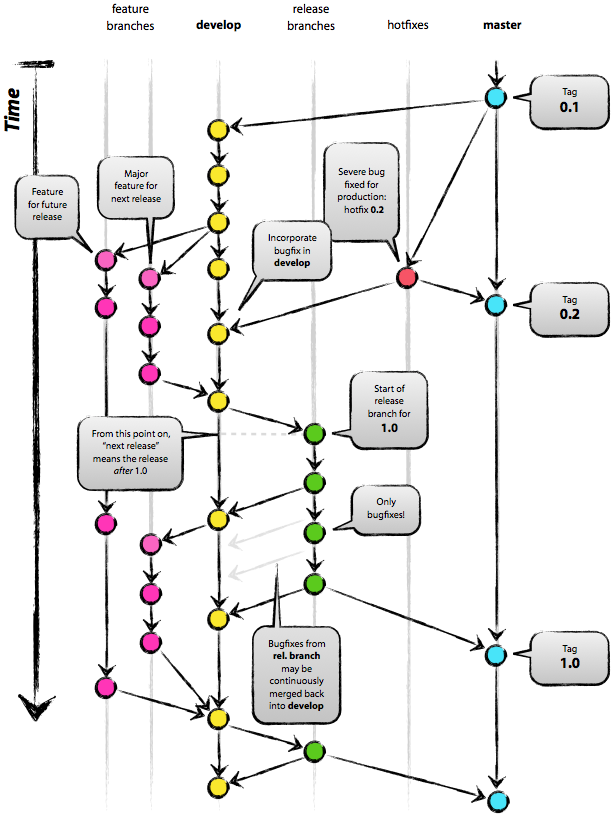
\includegraphics[width=120mm]{../Screenshots/gitflow.png}
					\caption{Branches are named at the top, and flow downwards}
					\label{fig:GitFlow}
				\end{center}
			\end{figure}

			In our simplified form there is no need for development and release branches, we simply ensured that master is always stable and production ready (or in other words, playable), and all new features are worked on on separate branches.
			In this way, members are able to work autonomously on a feature, without worrying about merge conflicts or committing unstable code.
			For the sake of one source of integration, Matt was the only member who would merge branches into master.

			One issue we had to overcome that Git could not really assist with was Unity's scene files being binary.
			Since Git cannot merge binary files, manual merging is necessary.
			To avoid this painstaking process as much as possible, we created a special \texttt{Dev} folder, whose contents would never be committed to the Git repository.
			In this folder members could experiment with test scenes, and only when they were complete would Matt be contacted to merge the scene into the single master scene in which the game is held.

			Thanks to our effective use of git, if in the future multiple parties wanted to add some of the content suggested previously in this section, they would need only to clone the repository, work on their desired changes in their own branch, and then submit a pull request to the Quantum Run repository maintainer.
			Even if these parties worked on similar areas, if they followed the systems we have set out earlier, conflicts should not be an issue.



\bibliography{references}{}
\bibliographystyle{plain}

\chapter{Appendices}
	\begin{figure}[ht]
		\begin{center}
			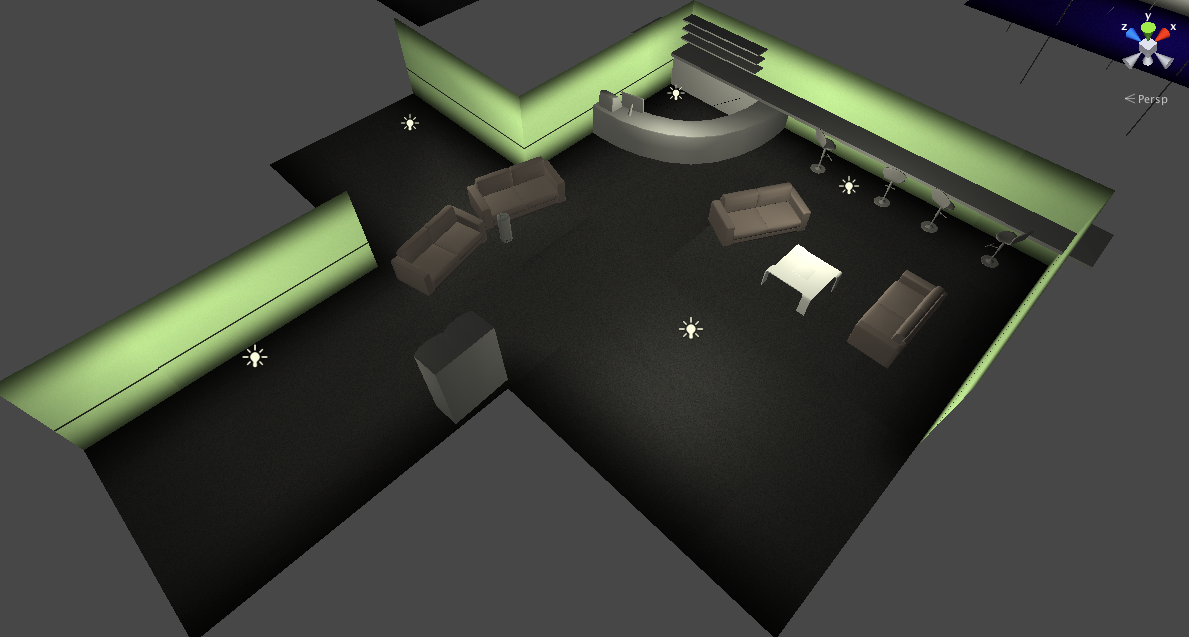
\includegraphics[width=150mm]{../Screenshots/Appendices/cafe.png}
			\caption{An example section nearing completion. Entirely modelled, textured, and lit by the team.}
		\end{center}
	\end{figure}

	\begin{figure}[ht]
		\begin{center}
			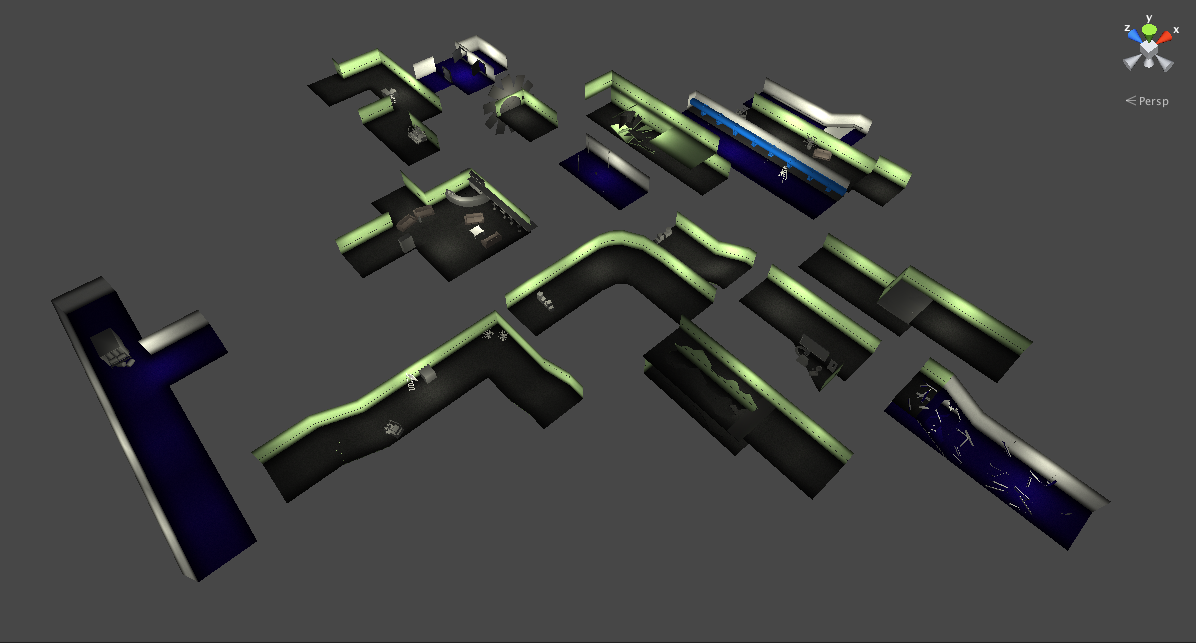
\includegraphics[width=150mm]{../Screenshots/Appendices/all-sections.png}
			\caption{Every section modelled and used in the final game.}
		\end{center}
	\end{figure}

	Figures ~\ref{fig:Algo1}, ~\ref{fig:Algo2}, and ~\ref{fig:Algo3} show birds eye view screenshots of the game level in three different runs. Note the significantly different level design caused each time.

	\begin{figure}[ht]
		\begin{center}
			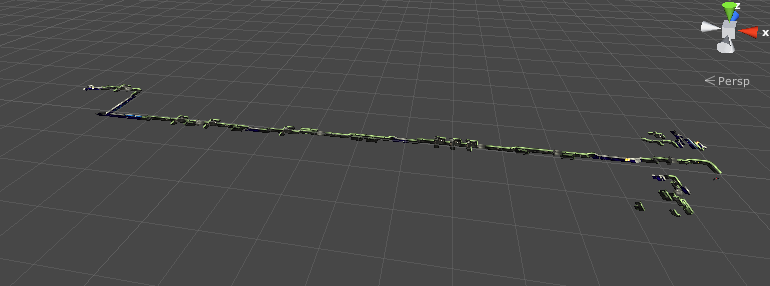
\includegraphics[width=150mm]{../Screenshots/Appendices/section_generation}
			\caption{Example 1 of the procedurally generated level algorithm in action.}
			\label{fig:Algo1}
		\end{center}
	\end{figure}

	\begin{figure}[ht]
		\begin{center}
			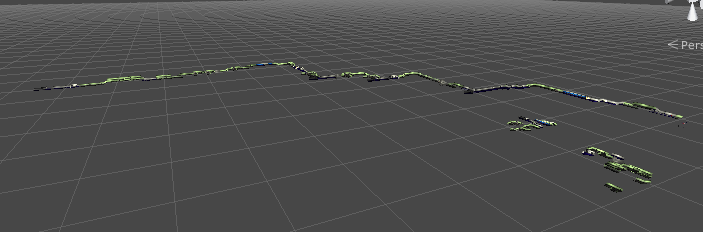
\includegraphics[width=150mm]{../Screenshots/Appendices/section_generation_2}
			\caption{Example 2 of the procedurally generated level algorithm in action.}
			\label{fig:Algo2}
		\end{center}
	\end{figure}

	\begin{figure}[ht]
		\begin{center}
			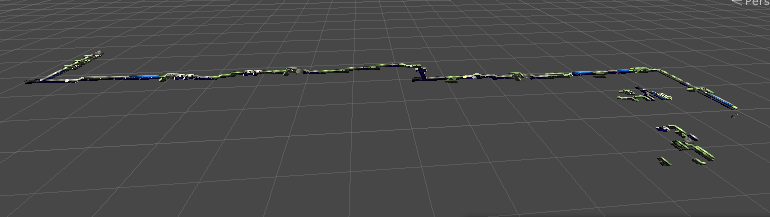
\includegraphics[width=150mm]{../Screenshots/Appendices/section_generation_3}
			\caption{Example 3 of the procedurally generated level algorithm in action.}
			\label{fig:Algo3}
		\end{center}
	\end{figure}

	\begin{figure}[ht]
		\begin{center}
			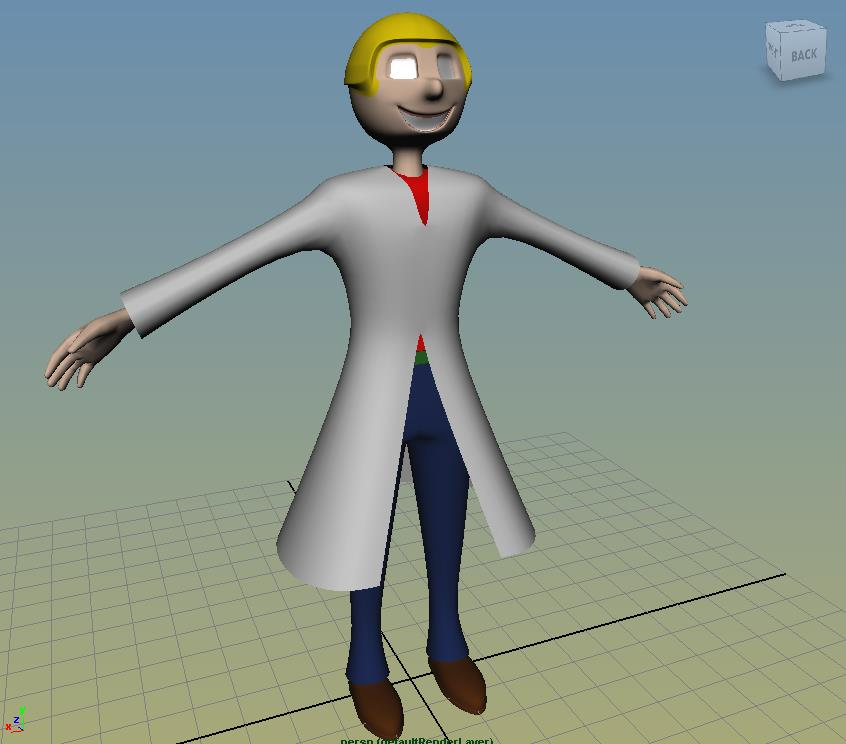
\includegraphics[width=150mm]{../Screenshots/Appendices/player-early}
			\caption{An early version of the player character.}
		\end{center}
	\end{figure}

	\begin{figure}[ht]
		\begin{center}
			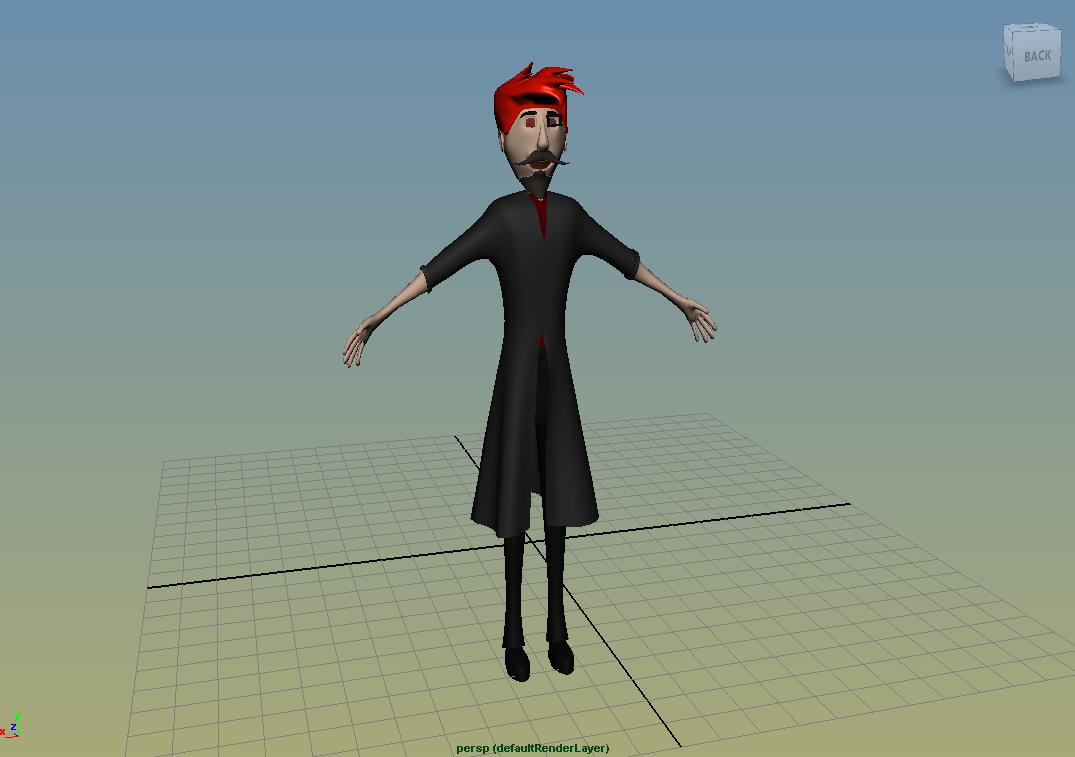
\includegraphics[width=150mm]{../Screenshots/Appendices/final-player-evil}
			\caption{The final design for the antimatter professor.}
		\end{center}
	\end{figure}

	\begin{figure}[ht]
		\begin{center}
			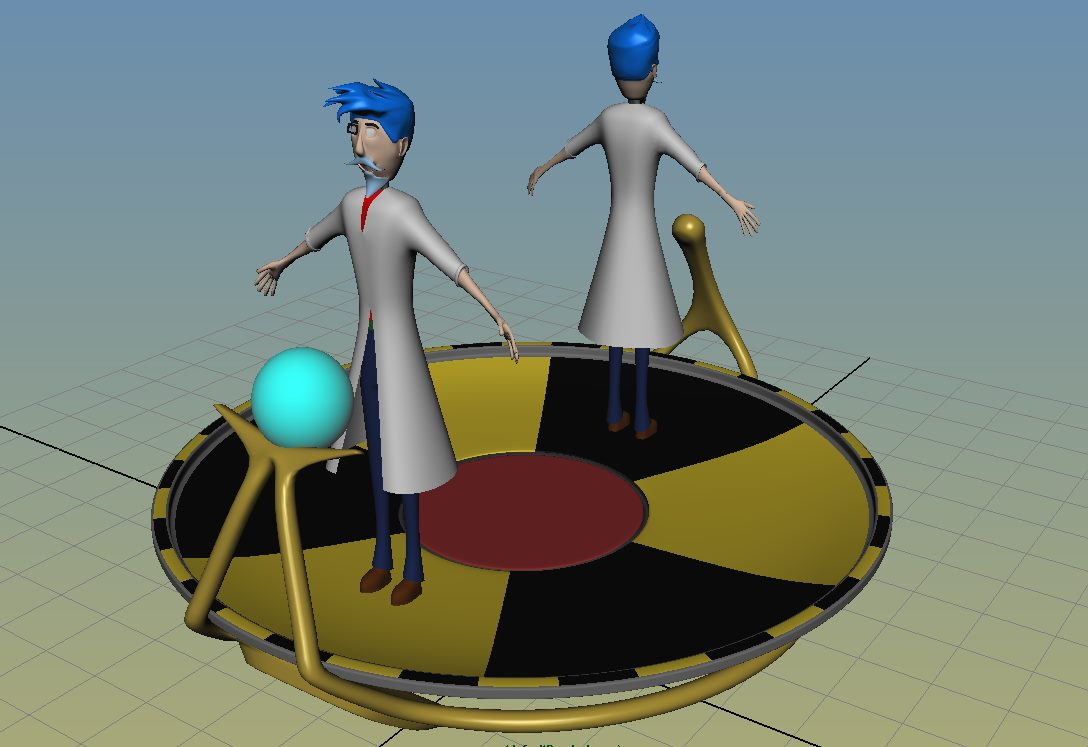
\includegraphics[width=150mm]{../Screenshots/Appendices/final-vehicle-design}
			\caption{The final design for the vehicle and players.}
		\end{center}
	\end{figure}

	\begin{figure}[ht]
		\begin{center}
			
\includegraphics[width=130mm]{../Screenshots/Appendices/lab-texture}
			\caption{The PSD texture for every lab section. Every wall, ceiling, and floor is mapped onto this one file.}
		\end{center}
	\end{figure}

	\begin{figure}[ht]
		\begin{center}
			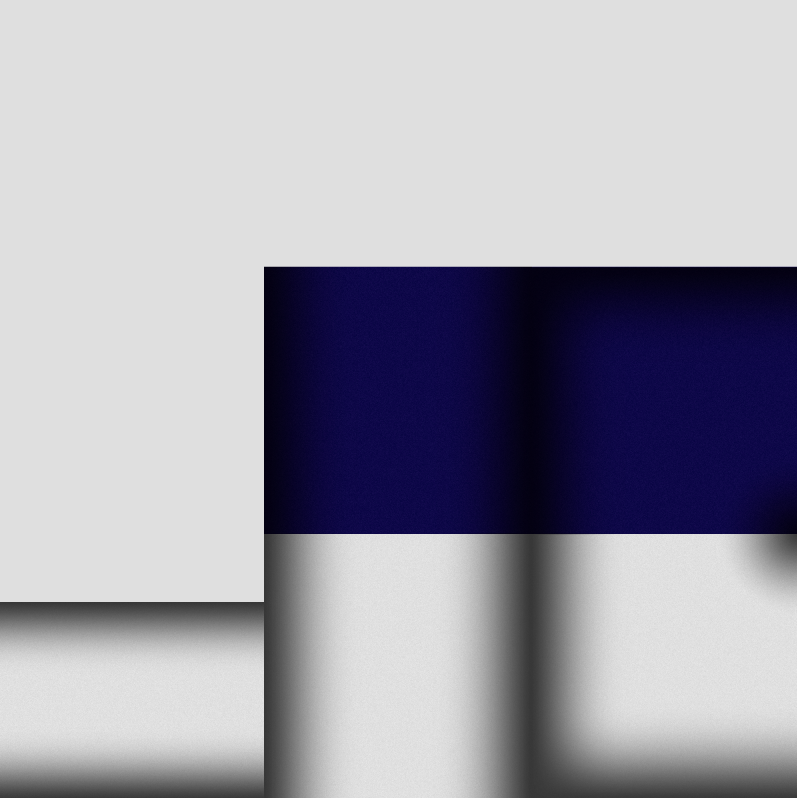
\includegraphics[width=130mm]{../Screenshots/Appendices/lhc-texture}
			\caption{The PSD texture for every LHC section. Every wall, ceiling, and floor is mapped onto this one file.}
		\end{center}
	\end{figure}

	\begin{figure}[ht]
		\begin{center}
			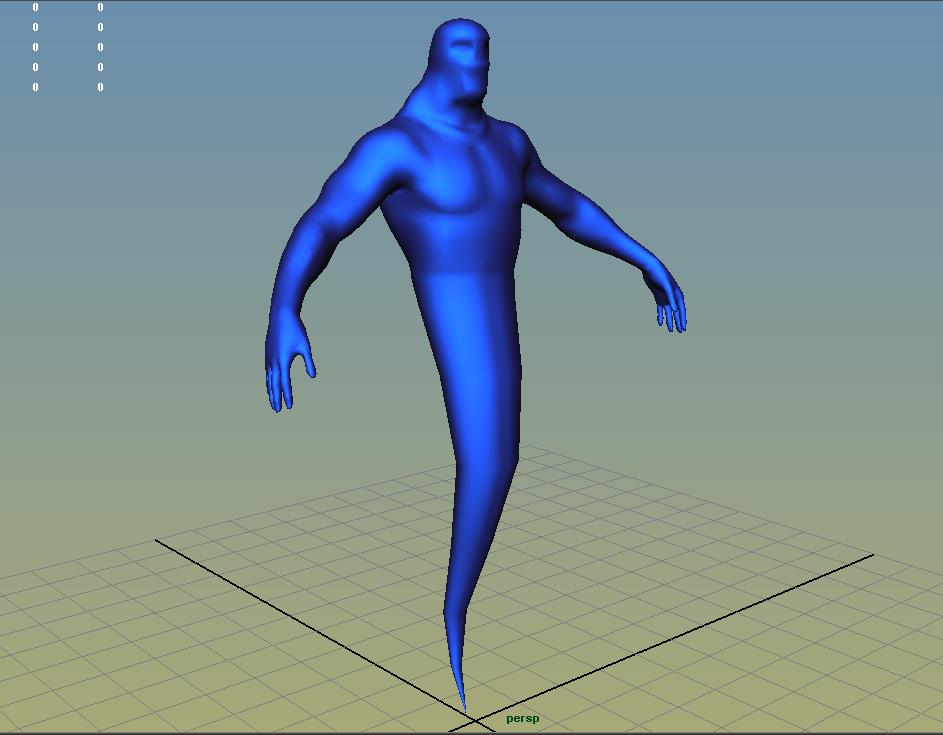
\includegraphics[width=150mm]{../Screenshots/Appendices/monster-early}
			\caption{An early iteration of the monster character.}
		\end{center}
	\end{figure}



\end{document}
